\documentclass{wptemp}
\usepackage{adjustbox}
\usepackage{setspace}\doublespacing%\onehalfspacing
\usepackage{natbib}
\newcommand{\GG}[1]{}
\usepackage{booktabs}
\usepackage{makecell}
\usepackage{siunitx}
\newcolumntype{d}{S[input-symbols = ()]}\singlespacing
\doublespacing
\usepackage{lscape}
\newcommand{\ts}{\textsuperscript}
\usepackage{threeparttable}
\usepackage{threeparttablex}

% *****************************************************************
% Estout LaTeX wrapper
% *****************************************************************

%%Original code developed by Jörg Weber: see
%% https://www.jwe.cc/2012/03/stata-latex-tables-estout/
%% and
%% https://www.jwe.cc/blog/



\let\estinput=\input % define a new input command so that we can still flatten the document

\newcommand{\estwide}[3]{
		\vspace{.75ex}{
			%\textsymbols% Note the added command here
			\begin{tabular*}
			{\textwidth}{@{\hskip\tabcolsep\extracolsep\fill}l*{#2}{#3}}
			\toprule
			\estinput{#1}
			\bottomrule
			\addlinespace[.75ex]
			\end{tabular*}
			}
		}	

\newcommand{\estauto}[3]{
		\vspace{.75ex}{
			%\textsymbols% Note the added command here
			\begin{tabular}{l*{#2}{#3}}
			\toprule
			\estinput{#1}
			\bottomrule
			\addlinespace[.75ex]
			\end{tabular}
			}
		}

% Allow line breaks with \ in specialcells
\newcommand{\specialcell}[2][c]{%
    \begin{tabular}[#1]{@{}c@{}}#2\end{tabular}
}

\newcommand{\sym}[1]{\rlap{#1}}% Thanks David Carlisle


%%%%%%%%%%% End of wrapper %%%%%%%%%%%%%%%%%%%%%
    
%%%%%%%%%%% TiKz %%%%%%%%%%%%%%%%%%%%%
\usepackage{tikz}
\usetikzlibrary{shapes.geometric, arrows}

\tikzstyle{startstop} = [rectangle, rounded corners, minimum width=3cm, minimum height=1cm,text centered, draw=black, fill=red!30]

\tikzstyle{io} = [trapezium, trapezium left angle=70, trapezium right angle=110, minimum width=3cm, minimum height=1cm, text centered, text width =5cm, draw=black, fill=blue!30]

\tikzstyle{process} = [rectangle, minimum width=3cm, minimum height=1cm, text centered, text width =5cm, draw=black, fill=orange!30]

\tikzstyle{decision} = [diamond, minimum width=3cm, minimum height=1cm, text centered, draw=black, fill=green!30]

\tikzstyle{arrow} = [thick,->,>=stealth]

\begin{document}

\linespread{1}{\title{{\fontfamily{ptm}\selectfont{\Large{\MakeUppercase{Democracy and Ethnic Favoritism: Evidence \\
from Africa}}}}\thanks{I am so grateful to Willa Friedman for her advice, comments and support. I thank Nathan Canen, Aimee Chin, German Cubas, Chinhui Juhn, Vikram Maheshri and the participants of the Empirical Microeconomics Workshop at the University of Houston for their comments and feedback. Abhi Basvoju provided excellent research assistance.}
}
}
	\author{{\fontfamily{pbk}\selectfont\large{\textsc{Hussain Hadah}}\thanks{Department of Economics, University of Houston, Science Building 3581 Cullen Boulevard Suite 230, Houston, TX 77204-5019, United States (e-mail: \email{hhadah@uh.edu}).}}}
	\date{\fontfamily{pbk}\selectfont\normalsize{\textsc{\today}}}
	\maketitle

\begin{center}
\href{https://hhadah.github.io/ethnicfavoritism/my_paper/HussainHadahEthFav.pdf}{\textcolor{green!15!black!30!blue}{\footnotesize{\textsc{Click Here to Get the Most Updated Version}}}}
\end{center}

\begin{abstract} 
What is the effect of democracy on ethnic favoritism? I estimate the relationship between co-ethnicity and five outcomes of public good provision – education, infant health, wealth, access to clean drinking water and access to electricity – using data from twenty-one African countries. Following previous research, I use variation in co-ethnicity across ethnic groups and over time. I first estimate the relationship between these five outcomes and co-ethnicity in the full sample and then split the analysis between anocracies and democracies. I find mixed evidence of ethnic favoritism in the full sample. I find more evidence of co-ethnic targeting when comparing within democracies only and within anocracies only.

\keywords{Ethnic favoritism; democracy; dictatorships; institutions.}
\JEL{D3, O1, O2.}
\end{abstract}

\thispagestyle{empty}
\clearpage
\pagenumbering{arabic}
	
\section{Introduction}

Ethnic favoritism has been widespread in Africa, and it negatively affects growth. One example of such action was from Zimbabwe, where the White minority ruled the country after independence. During colonization and following independence in the short-lived Rhodesia, Whites enjoyed special privileges. They were also granted free agricultural farms. Policies that favored a specific ethnic group created an economic gap between White and Black Zimbabweans. Even though Whites accounted for 0.3\% of the population, they owned 70\% of the farming land \citep{batha_2000}. Ethnic diversity could lead to lower growth as a result of conflicts and rent-seeking by politically dominant ethnic groups. \citet{la1999quality}, \citet{alesina1999public}, \citet{alesina2003fractionalization} and \citet{alesina2011segregation} show that ethnic fractionalization and ethnic segregation affects the quality of governance and creates conflicts over the provisions of public goods. Ethnic diversity also affect the productivity of labor \citep{ lazear1999culture, habyarimana2007does, hjort2014ethnic}. \citet{francois2015power} show that African leaders share the benefits of heading an ethnically diverse country among ministers from different ethnic groups to maximize their time in power. Instances like these could explain the inequality among the ethnic lines and why Africa lags behind economically and in public goods provisions \citep{easterly1997africa, alesina2005ethnic, miguel2005ethnic, glennerster2013collective}.  \citet{golden2013distributive}, in a review of ethnic favoritism empirical studies, show that the majority of papers study ethnic favoritism in one democratic country or focus on one outcome.  Understanding the effect of political systems on the persistence of ethnic favoritism is essential in understanding Africa's economic development. I aim to answer the following question. Do democratic institutions affect the prevalence of ethnic favoritism?

This paper makes two contributions to the literature. First, it investigates the existence of ethnic favoritism on a few outcomes---schooling, infant suvival, wealth, electrification and access to clean drinking water---that are essential for economic development. Second, it provides empirical evidence from a sample of many countries on the existence of differential co-ethnic effects between countries that are more or less democratic.

What causes some countries to distribute resources evenly among their citizens while others take a different path that benefits a specific ethnic group? What stops a leader from favoring their ethnic kins? The literature of ethnic favoritism is rife with research on the existence of the phenomena \citep{friedman2018corruption, franck2012does, hodler2014regional, kramon2013benefits}. \citet{friedman2018corruption} found that Kenyans that are of the same ethnicity as the leader disproportionately received antiretroviral drugs. \citet{franck2012does} studied the effect of ethnic favoritism in health and education in multiple African countries. They found that the leader's ethnic group is more likely to complete primary school and have better health outcomes. \citet{kramon2013benefits} found that ethnic favoritism in education exists in Africa. \citet{kasara2007tax} finds that African leaders tax their ethnic group more because they can exert more control over them. Suggesting that ethnic groups do not benefit from having ethnic kin in power. \citet{kudamatsu2009ethnic} exploits an exogenous change in the ethnicity of the president of Guinea to study ethnic favoritism on infant mortality. They find that the ethnic group of the president did not enjoy an advantage in the reduction of infant mortality.\footnote{\citet{kudamatsu2012has}, they studied the effect of democratization on infant mortality. They find that democratization reduced infant mortality by 1.2 percentage points.} Distributive policies that favor one group over another are not exclusive to developing countries. \citet{goss1972military} documented how the members of the principal military committees in the United States received unrepresentative constituency benefits. \citet{ferejohn1974pork}  shows that influence in congress and pork barrels over rivers and harbors are distributed based on political consideration and not improving the public good.

Therefore, all of these papers looked at the existence of ethnic favoritism in several countries. However, they did not attempt to find a relationship between ethnic favoritism and democracy, which I aim to do in this paper.

Others tried to investigate the presence of ethnic favoritism during periods of democracy in a specific country \citep{burgess2015value, dionne2016political, harris2019under, kramon2016ethnic}. \citet{harris2019under} found that members of the Kenyan parliament do not disproportionally favor their constituents. \citet{burgess2015value} also tried to find the effect of democracy on ethnic favoritism in Kenya using data on road building. They found that ethnic favoritism exists in Kenya, but it disappears during periods of democracy. \citet{amodio2016ethnic} investigated ethnic favoritism toward the Zulu nation in South Africa when it was a new democracy. They found that when the Zulu-based Inkatha Freedom Party (IFP) is in the majority, Zulu individuals experience better labor market outcomes. \citet{dionne2016political} also tried to investigate the existence of ethnic favoritism in agricultural subsidies in Malawi. They found that the incumbent majority party, at the time, Democratic Progressive Party headed by president Bingu wa Mutharika did not systematically target the ethnic kins of Mutharika and their co-partisans. The analysis of this group of papers was limited to one or two countries. Therefore, they did not have enough observations of transitions from democracy to dictatorship and \textit{vice versa}. For example, in \citet{burgess2015value}, Kenya changed its political system twice. Thus, the analysis was technically restricted to two observations over time. I try to circumvent this problem in this paper by taking into consideration 21 countries that transitioned into and out of democracy twenty times.

Moreover, using a continuous democracy index, Polity IV, I can observe changes in democratic institutions and run a heterogeneous effect analysis. For example, in 1991, Mali was transitioning from dictatorship to democracy. Using a dummy variable for democracy, I would observe that Mali became a democracy in 1992. However, by using Polity IV, I found that in 1990, Mali's \textit{Polity} score was -7, which increased to 4 in 1992 then 5 in 1997. 

Additionally, the literature considered the effects of institutions on economic growth. This relates to the topic I propose because a democratic system is contained in the group of all institutions. \citet{alsan2015effect} looked for a link between the prevalence of the Tse Tse fly in Africa and how it affected institution building. She found that the fly impeded a society's ability to settle down and build institutions. Therefore, it put these countries on a lower growth trajectory. \citet{acemoglu2001colonial} tried to measure institutions using the number of European Colonial fatalities as an instrumental variable. The authors found that countries with a  more hospitable environment toward European settlers had better institutions than those that were not. They also found that the European mortality rate was negatively correlated with economic growth. In other words, countries with a high European mortality rate had a worse economic performance than those that did not. My paper would add to this literature by studying the effect of democratic institutions on ethnic favoritism that holds Africa back from growing faster. 

Ethnic favoritism has played a role in political economy theories. \citet{fearon1999ethnic} and \citet{caselli2006theory} introduced theories in which ethnicity is a tool of exclusion and to enforce coalition membership. \citet{francois2015power} introduced a model of power-sharing in Africa. They show that African countries, mainly autocracies, appoint a cabinet in a manner that represents the ethnic diversity of the population. More precisely, they find that large ethnic groups are slightly underrepresented, minorities are overrepresented and the leader's ethnic group has a slight premium. The leader, in return, distributes the benefits of being in power among the ministers to stay in power. \citet{padro2007control} show that patronage, taxation and spending change with changes in the ethnic group in power, which contributes to bad governance, ethnic bias and wasteful policies in Africa.


The literature lacks an empirical framework to explain the differences in ethnic bias among countries. Moreover, there is an even more significant gap investigating the existence of a link between democratic institutions and favoritism across nations. In this paper, I examine ethnic favoritism in twenty-one African countries and estimate its persistence during periods of democracy and dictatorship. 

Using data from the Demographics and Health Survey (DHS), I estimate the effect of ethnic favoritism and democracy on a few outcomes of interest such as education, wealth, infant survival, electrification and access to clean drinking water. Using a rich data set, I was able to control for ethnic group, time and age fixed effects. 

There are several tools that a leader could use to benefit the educational, health, wealth and infrastructure outcomes of their ethnic kins. Leaders could hire more teachers, improve the physical health of schools \citep{glewwe2006schools} or waive fees and pay people to go to school. A leader could also improve access to immunization and antiretroviral drugs and increase the transfers to the health care sector \citep{friedman2018corruption, jones2003many}. A leader could also improve the status of infrastructure, water and electricity, by favoring regions that are populated by their own ethnic group \citep{hodler2014regional}.

Another way that a leader could improve the fortune of their ethnic group is by offering government jobs to them. By offering more public sector jobs to members of their group, the leader is decreasing unemployment among their group and increasing their wealth and income. An increase in income could in return affect the health and education outcomes of the ethnic group. Families, in this situation, are more likely to afford health care and to send their children to schools. 

Figure \ref{fig:coeet} and table \ref{tab:eth} summarize the effect of ethnic favoritism on education, wealth, infant survival, electrification and access to clean drinking water. People that spent all of their primary school when a leader was co-ethnic were 3.8 percentage points less likely to finish primary school, though the result was statistically insignificant. A child whose mom shared the same ethnicity as the leader of the country she lived in two years before birth is 0.5 percentage points more likely to survive the first 12 months of birth, the result was statistically insignificant. Co-ethnics were as likely as their non-co-ethnic peers to be in the same wealth quintile and to have access to clean drinking water. Co-ethnics were 4.2 percentage points more likely to have electricity. 

Figure \ref{fig:coedemet} and table \ref{tab:ethdem} summarize the effect of co-ethnicity on the outcomes of interest once I allow for the heterogeneous effect of democracy. The interaction between democratic bins and co-ethnicity is statistically significant when studying their effect on electrification and access to clean drinking water.\footnote{Democratic bins include a bind for democracies with a polity score between 10 and 5, anocracies with a polity score between 5 and -5, and dictatorships with a polity score less than -5.} Co-ethnicity and more democracy do not eliminate ethnic favoritism when it comes to primary school completion, infant survival and wealth. Co-ethnics in democracies are as likely to finish primary schooling, survive the first year of birth and belong to the same wealth quintile as their non-co-ethnic peers. Co-ethnics in anocracies are 3.3 percentage points more likely to finish primary schooling but are as likely to survive the first year of birth and belong to the same wealth quintile as their non-co-ethnic peers.  However, Co-ethnics in democracies are 15.4 percentage points more likely to have access to electricity. Co-ethnics in anocracies are 6.7 percentage points more likely to have access to electricity. Finally, co-ethnics in both democracies and anocracies are more likely to have better access to clean drinking water.

The rest of this paper will be divided into four sections. I will discuss the theoritical framework in Section \ref{sec1}, section \ref{sec2} will be on the data and the construction of the co-ethnic leader variable. Sections \ref{sec4}, \ref{sec5}, and \ref{sec6} will respectively layout an empirical model, discuss the results and then conclude. 

\section{Theoretical Framework}\label{sec1}
\subsection{Ethnic Favoritism Models}
The literature on ethnic favoritism provides us with a few models that explain the existence of the phenomena \citep{cox1986electoral, dixit1996determinants, lindbeck1987balanced}. I will discuss these models and offer implication that arises from them.

\citet{cox1986electoral} present a  model where they assume that a leader's utility is directly affected by the well-being of their ethnic kins. The strong assumption they make will steer a leader to favor their ethnic group regardless of the group's political behavior. In other words, a president of a country will always be allocated funds to favor their ethnic group even if they do not vote for them. This is referred to as the ``ethnic altruism" model.

\citet{dixit1996determinants} assume that a leader's only objective is to maximize time in power. In this model, a leader will transfer funds to several groups, not only their own, to increase public support. They also assume that ethnic kins get utility from the mere fact that a co-ethnic person is holding high office. This is referred to as the ``psychic benefit" \citep{chandra2007ethnic}. The psychic benefit model provides an important implication: members of an ethnic group will give unequivocal support to a co-ethnic leader even if they do not get anything in return. Under this scenario, a leader will have no incentives to favor their ethnic group, therefore, ethnic favoritism will not exist. This model is inconsistent with the empirical evidence that shows the existence of ethnic favoritism.

Finally, \citet{lindbeck1987balanced} established a model wherein a leader is an office-seeker. The office-seeking behavior requires political support. They drop the ``psychic benefit" assumption. In this model, an ethnic group will only support a co-ethnic leader if she/he provides them with material benefits, like schools and roads. A leader will support their ethnic groups for two reasons. First, it could be the case that the support of the co-ethnic group is cheaper than other groups. The lower cost of allocating funds comes from the fact that the leader understands the needs of their ethnic group and is better at allocating resources to meet these needs. Second, if a leader is risk-averse, then they will trust the promises that their ethnic group will support them more than the other ethnicities. Therefore, it is less risky for them to buy the support of their group in exchange for benefits. This is called the \textit{quid pro quo} model.

There are several tools that a leader could use to benefit the educational, health, wealth and infrastructure outcomes of their ethnic kins. Leaders could hire more teachers, improve the physical health of schools \citep{glewwe2006schools} or waive fees and pay people to go to school. A leader could also improve access to immunization and antiretroviral drugs and increase the transfers to the health care sector \citep{friedman2018corruption, jones2003many}. A leader could also improve the status of infrastructure, water and electricity, by favoring regions that are populated by their own ethnic group \citep{hodler2014regional}.

Another way that a leader could improve the fortune of their ethnic group is by offering government jobs to them. By offering more public sector jobs to members of their group, the leader is decreasing unemployment among their group and increasing their wealth and income. An increase in income could in return affect the health and education outcomes of the ethnic group. Families now could afford health care and send their children to schools. 

The theory on ethnic favoritism yields different results under different assumptions. These conclusions are in contrast with the empirical evidence that shows that ethnic favoritism exists. Therefore, testing for ethnic favoritism using different data sets, countries and analyses remains an important contribution to the literature of ethnic favoritism.

\section{Data}\label{sec2}
The data I am using is from twenty-one African countries spanning the period from 1947 to 2000. I present the summary statistics of the sample in table \ref{tabsum}.

\subsection{Demographics and Health Survey}
The Demographics and Health Survey (DHS) is a nationally representative survey conducted in over 90 countries. It aims to improve the understanding of global development. The United States Agency for International Development, known as USAID, funds the DHS project. In their surveys, they collect a myriad of significant variables in measuring a country's development. Moreover, the female and male surveys collect detailed information, like schooling, access to water, and ethnicity, that are important in estimating ethnic favoritism. Since ethnicity is more salient in African countries, I will limit my data to the continent \citep{murphree1988salience, posner2004political}. Out of the African countries surveyed by the DHS, I excluded the ones where ethnic information was not collected. For example, in Burundi, the DHS only asked a question about the nationality of the interviewee.

By merging this data set with other data that I am using, I will create a few databases consisting of between $822,347$ and $2,651,752$ observations from twenty-one countries. Moreover, the data include cohorts that were born between $1947$ to $2000$. I introduce the summary statistics in table \ref{tabsum}. The average age was $29$, and females in the sample had an average of $2.94$ children. On average, a household consisted of $7.3$ members. Access to electricity and wealth index are measures of well-being.\footnote{The wealth index is a value of standardized scores and factor coefficient scores of wealth indicators.} $19\%$ of the sample belong to the poorest wealth quintiles. Only $31\%$ of the people surveyed had access to electricity. The mean total years of education was about $5$ years.

\begin{table}

\caption{Summary Statistics \label{tabsum}}
\centering
\begin{threeparttable}
\resizebox{\linewidth}{!}{
\fontsize{7}{9}\selectfont
\begin{tabular}[t]{lcc}
\toprule
\multicolumn{1}{c}{ } & \multicolumn{1}{c}{\textbf{Men and Women Recode}} & \multicolumn{1}{c}{\textbf{Children Recode}} \\
\cmidrule(l{3pt}r{3pt}){2-2} \cmidrule(l{3pt}r{3pt}){3-3}
\textbf{Characteristic} & \textbf{N = 1,387,301} & \textbf{N = 2,801,526}\\
\midrule
Age & \makecell[c]{29 \\(10) } & \\
Total children ever born & \makecell[c]{2.94 \\(2.87) } & \\
Total number of household members & \makecell[c]{7.3 \\(5.0) } & \\
Has electricity & 0.31 & \\
Currently working & 0.55 & \\
Wealth Quintile &  & \\
\hspace{1em}1 & 0.19 & \\
\hspace{1em}2 & 0.18 & \\
\hspace{1em}3 & 0.19 & \\
\hspace{1em}4 & 0.20 & \\
\hspace{1em}5 & 0.24 & \\
Total years of education & \makecell[c]{5.0 \\(4.7) } & \\
Completed primary school & 0.65 & \\
Urban & 0.36 & \\
Literacy & 0.58 & \\
Infant Survival &  & 0.91\\
Current age of child in years &  & \makecell[c]{10 \\(7) }\\
Female Children &  & 0.49\\
Children’s total years of education &  & \makecell[c]{3.0 \\(3.9) }\\
\bottomrule
\end{tabular}}
\begin{tablenotes}
\item[1] Mean (Standard Deviation); \%.
\item[*] Data source is the Demographic and Health Surveys's (DHS) men, women, and children recodes.
\end{tablenotes}
\end{threeparttable}
\end{table}


\subsection{Democracy Data}
I use Polity IV \citep{marshall2019polity} as an indicator for democratic institutions and supplemented it with the Democracy-Dictatorship Index \citep{cheibub2010democracy}. Polity IV is an annual measure that scores each country, since its independence, from -10 to 10--- 10 being the most democratic and -10 the most autocratic. The scoring is based on five criteria: 
\begin{enumerate}
\item Competitiveness of the executive.
\item The openness of the executive.
\item Regulation of political participation. 
\item The competitiveness of political participation
\item Constraints on the executive branch. 
\end{enumerate}
The first two conditions are concerned with barriers to entry, or lack of, to become the leader of the executive branch (i.e., the president or prime minister). The easier it is for a person to enter the election, the more democratic the country. The third and fourth benchmarks focus on political life in a country. The less constrained a person's freedoms are, the more democratic the state. The final requirement relates to the amount of power a country's leader could yield. On the one hand, in the United States, the president's powers are checked by the legislative and judicial branches of government.
On the other hand, President Mobutu Sese Seko of the Democratic Republic of Congo ruled with an iron fist from 1965 till 1996. His powers were unchecked, and his decisions were undoubted. 

Moreover, I use the Democracy-Dictatorship Index to complement the data set and not as a primary source of data on democracy. I will also use the Democracy-Dictatorship to check the robustness of my results (see these results in table \ref{tab:ethdemdic} and figure \ref{fig:demdicindex}). The Democracy-Dictatorship Index \citep{cheibub2010democracy} has a list of the holders of countries' top two offices--- for example, president and vice president--- with their titles and source of power.\footnote{By source of power, I mean if a leader was elected or got into power through a coup.} For instance, Idi Amin of Uganda became president in 1971 through a coup d'etat. While Nelson Mandela, of South Africa, was the first South African to be elected in a free election in 1994. The average polity score in the data set was -4.75 (see table \ref{tabsum}). 

Furthermore, I present the evolution of democracy from 1980 to 2000 in figure \ref{fig1}. Notice how Ghana, with a score of 5, and Nigeria, with a score of 7, were the most democratic countries in 1980. During the 1980s, the apartheid state's repeal in South Africa had just begun, which explains the score of 4. By the year 2000, five countries--- Benin, Malawi, Namibia, Senegal, and South Africa--- were democracies. 

\begin{figure}[!htb]
\centering
\caption{Democracy in sample countries from 1980 to 2000.}
\label{fig1}
\begin{subfigure}{.48\textwidth}
\centering
\caption{Polity Scores in 1980.}
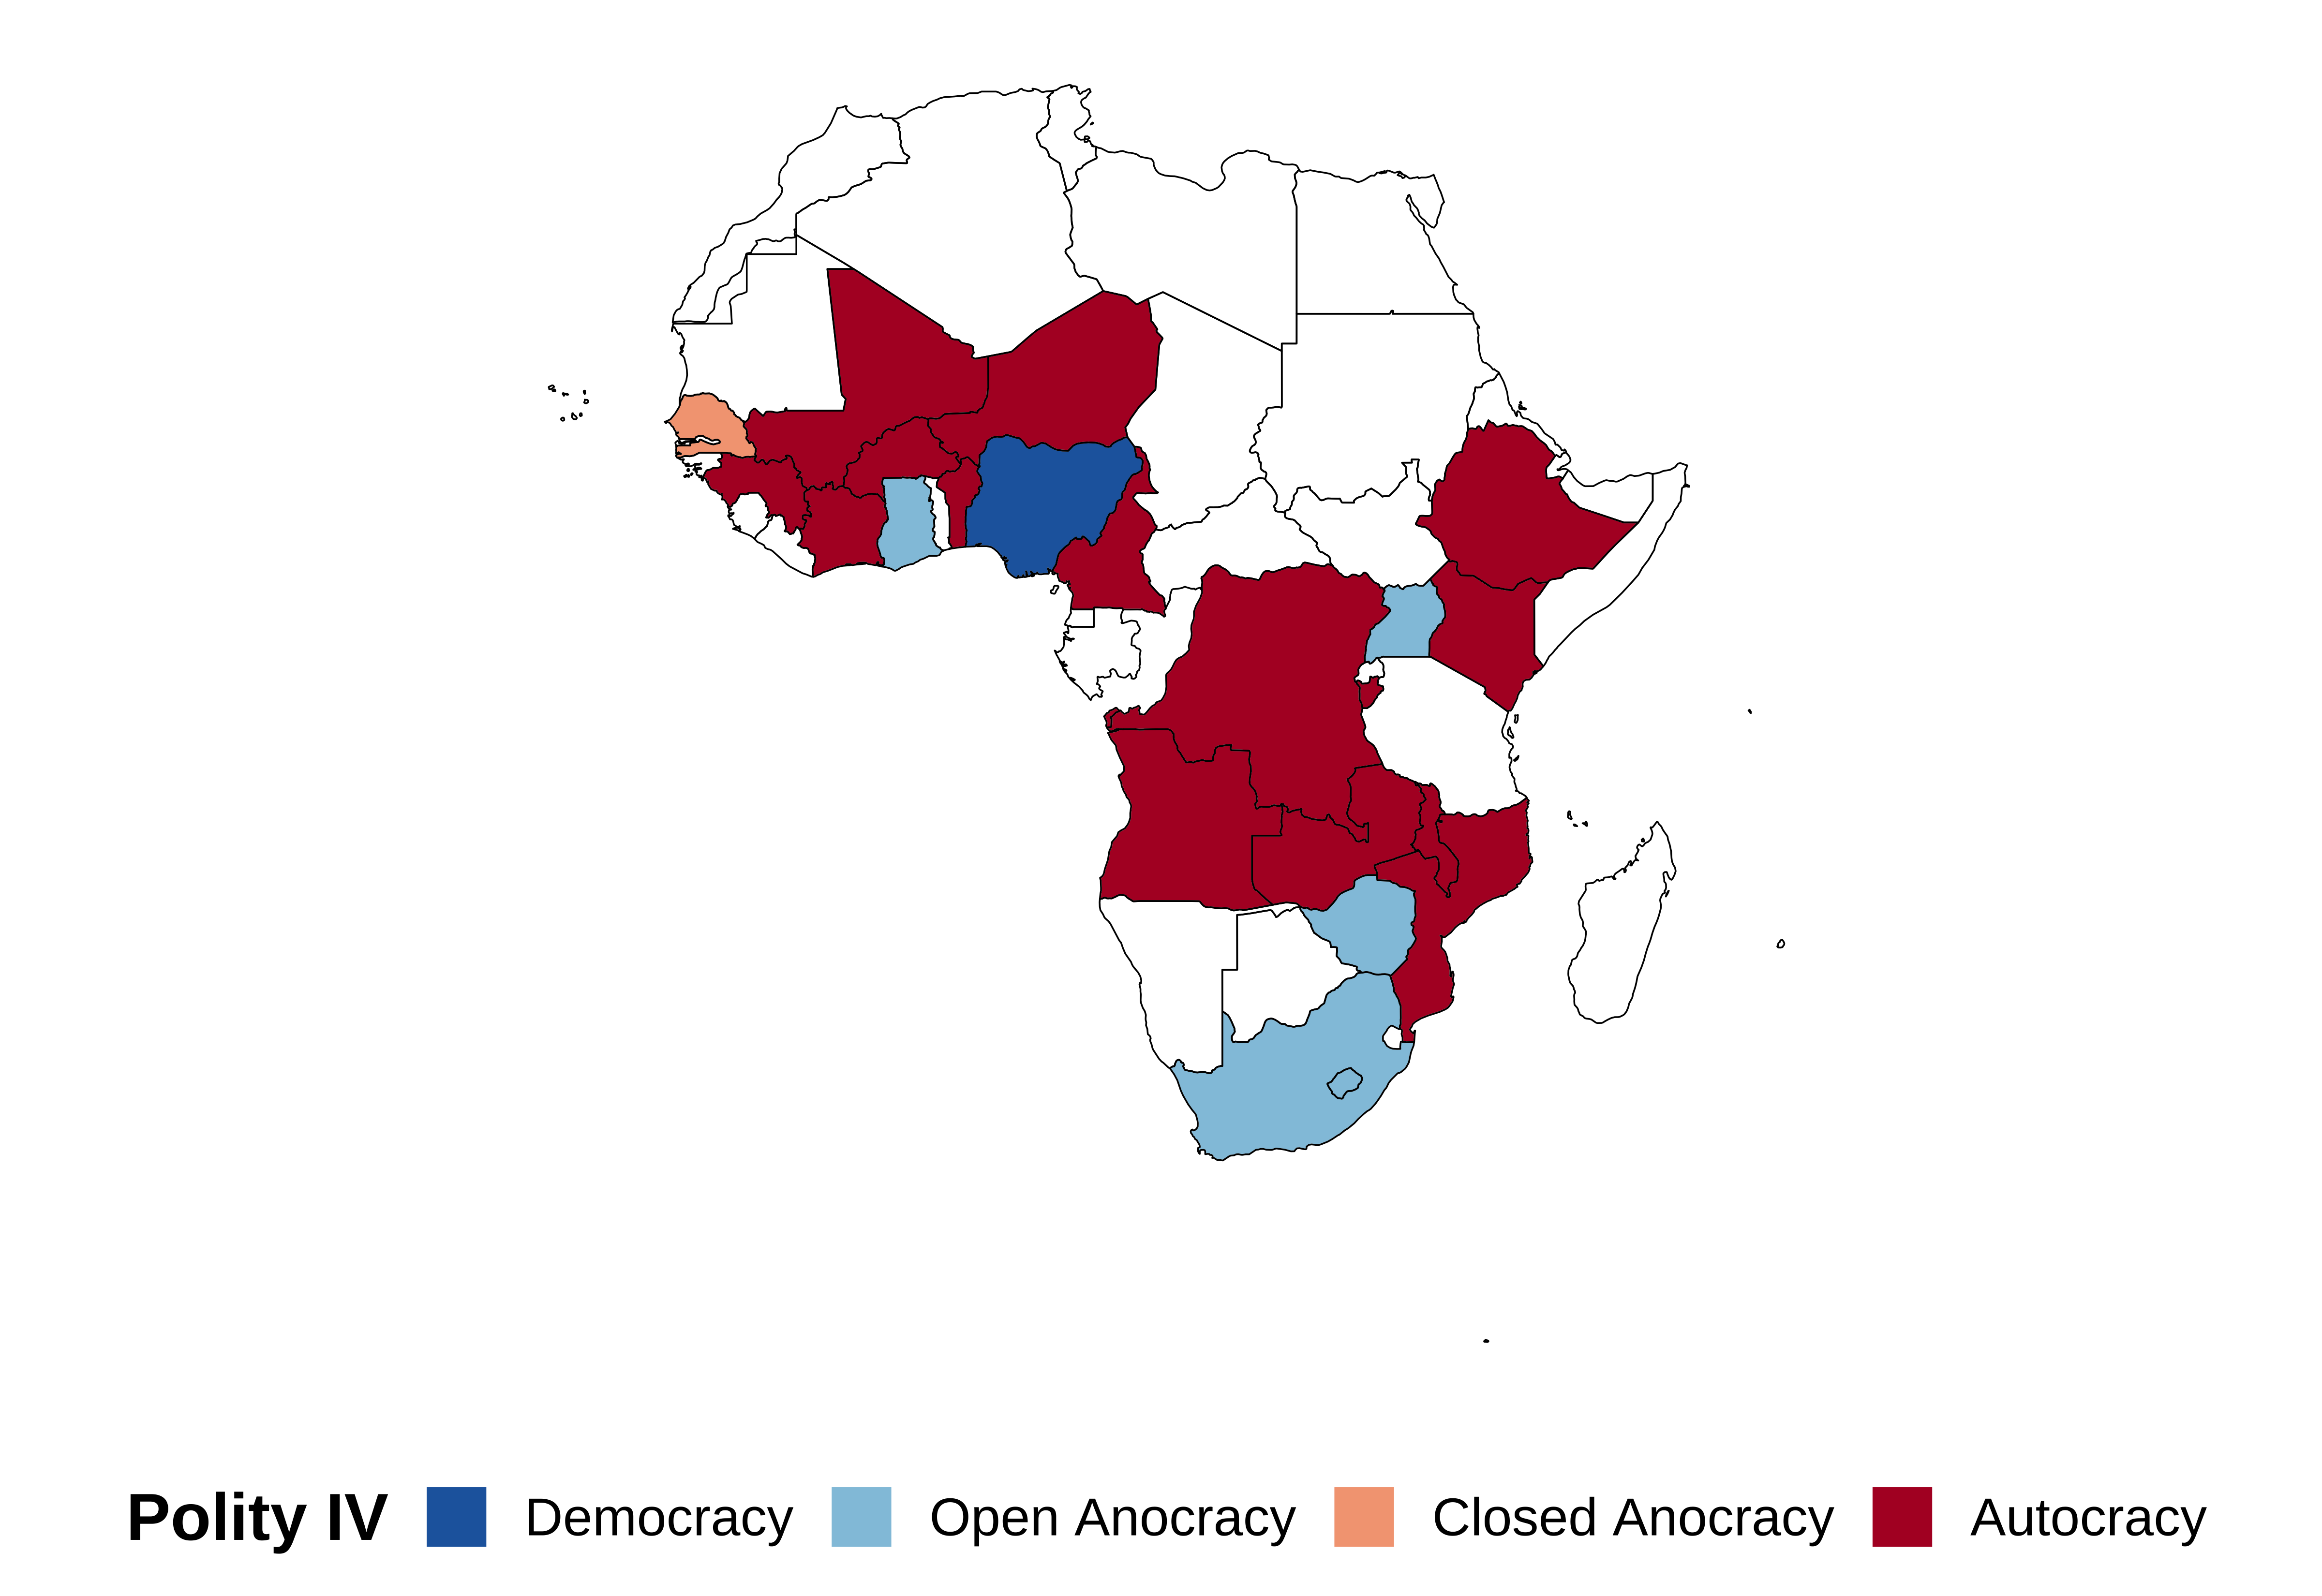
\includegraphics[width=.9\linewidth]{figure/1980.png}
\label{fig1980}
\end{subfigure}
\centering
%Second graph
\begin{subfigure}{.48\textwidth}
\centering
\caption{Polity Scores in 1985.}
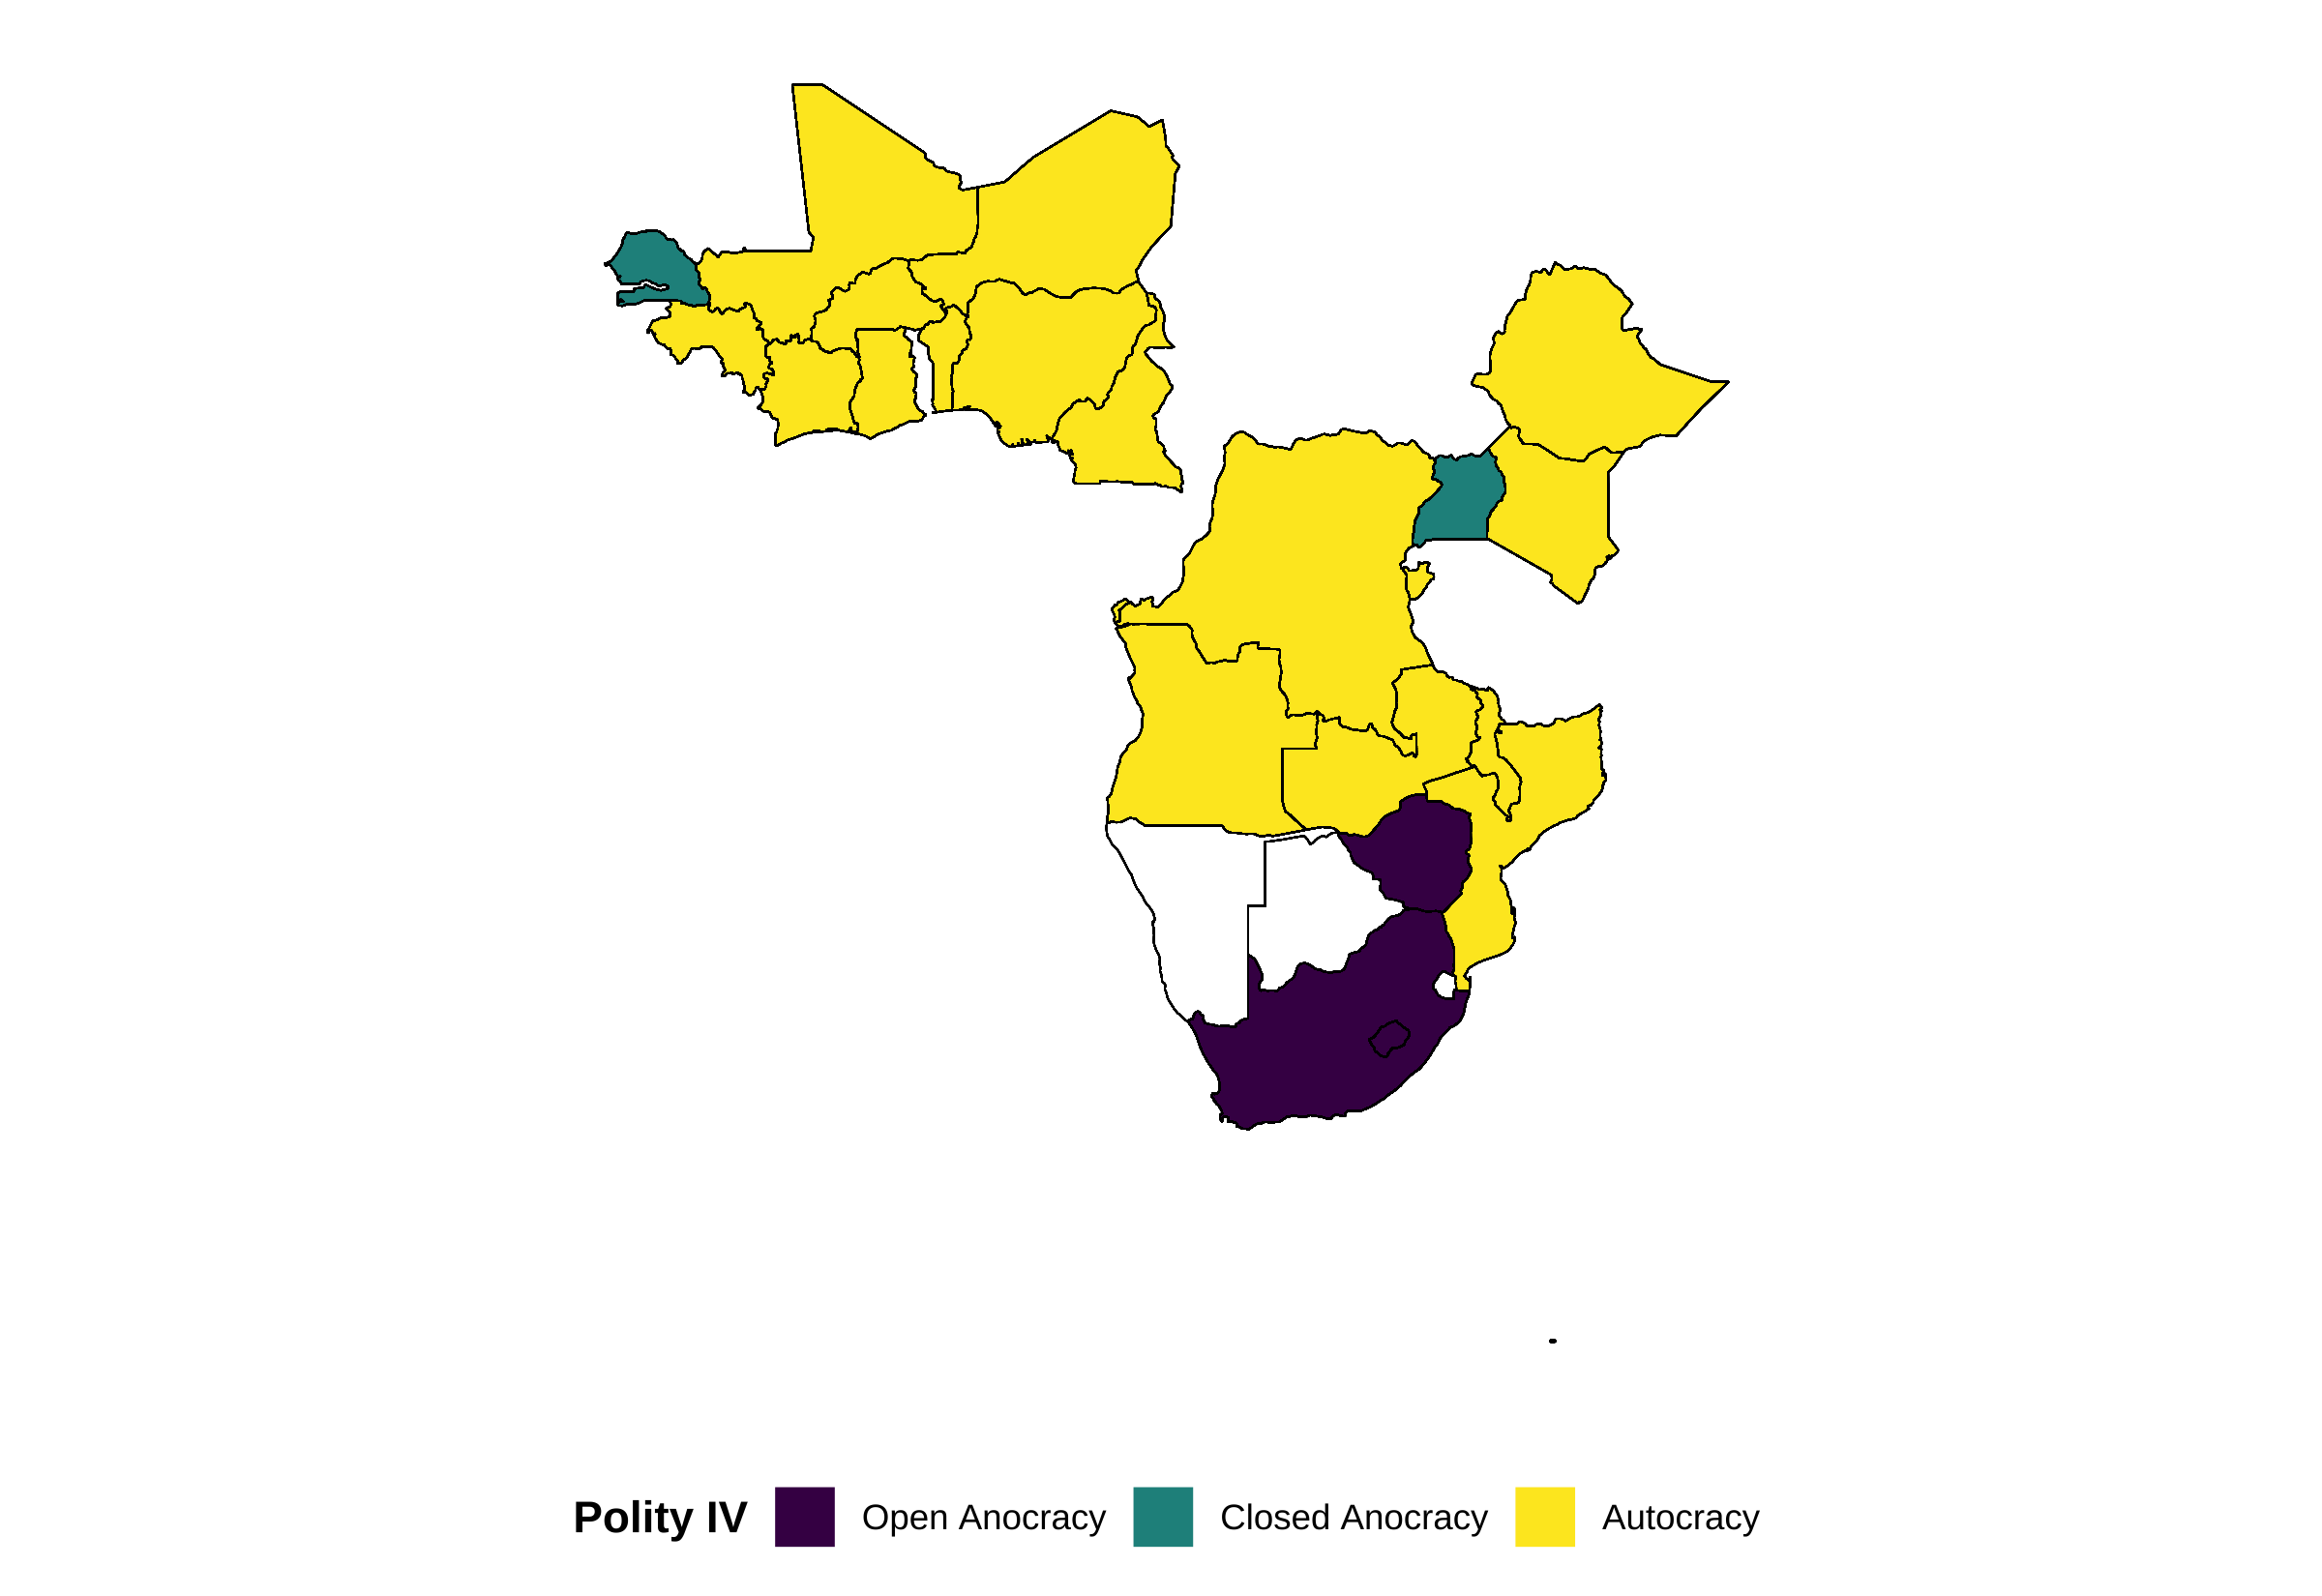
\includegraphics[width=.9\linewidth]{figure/1985.png}
\label{fig1985}
\end{subfigure}
%Third
\begin{subfigure}{.48\textwidth}
\centering
\caption{Polity Scores in 1990.}
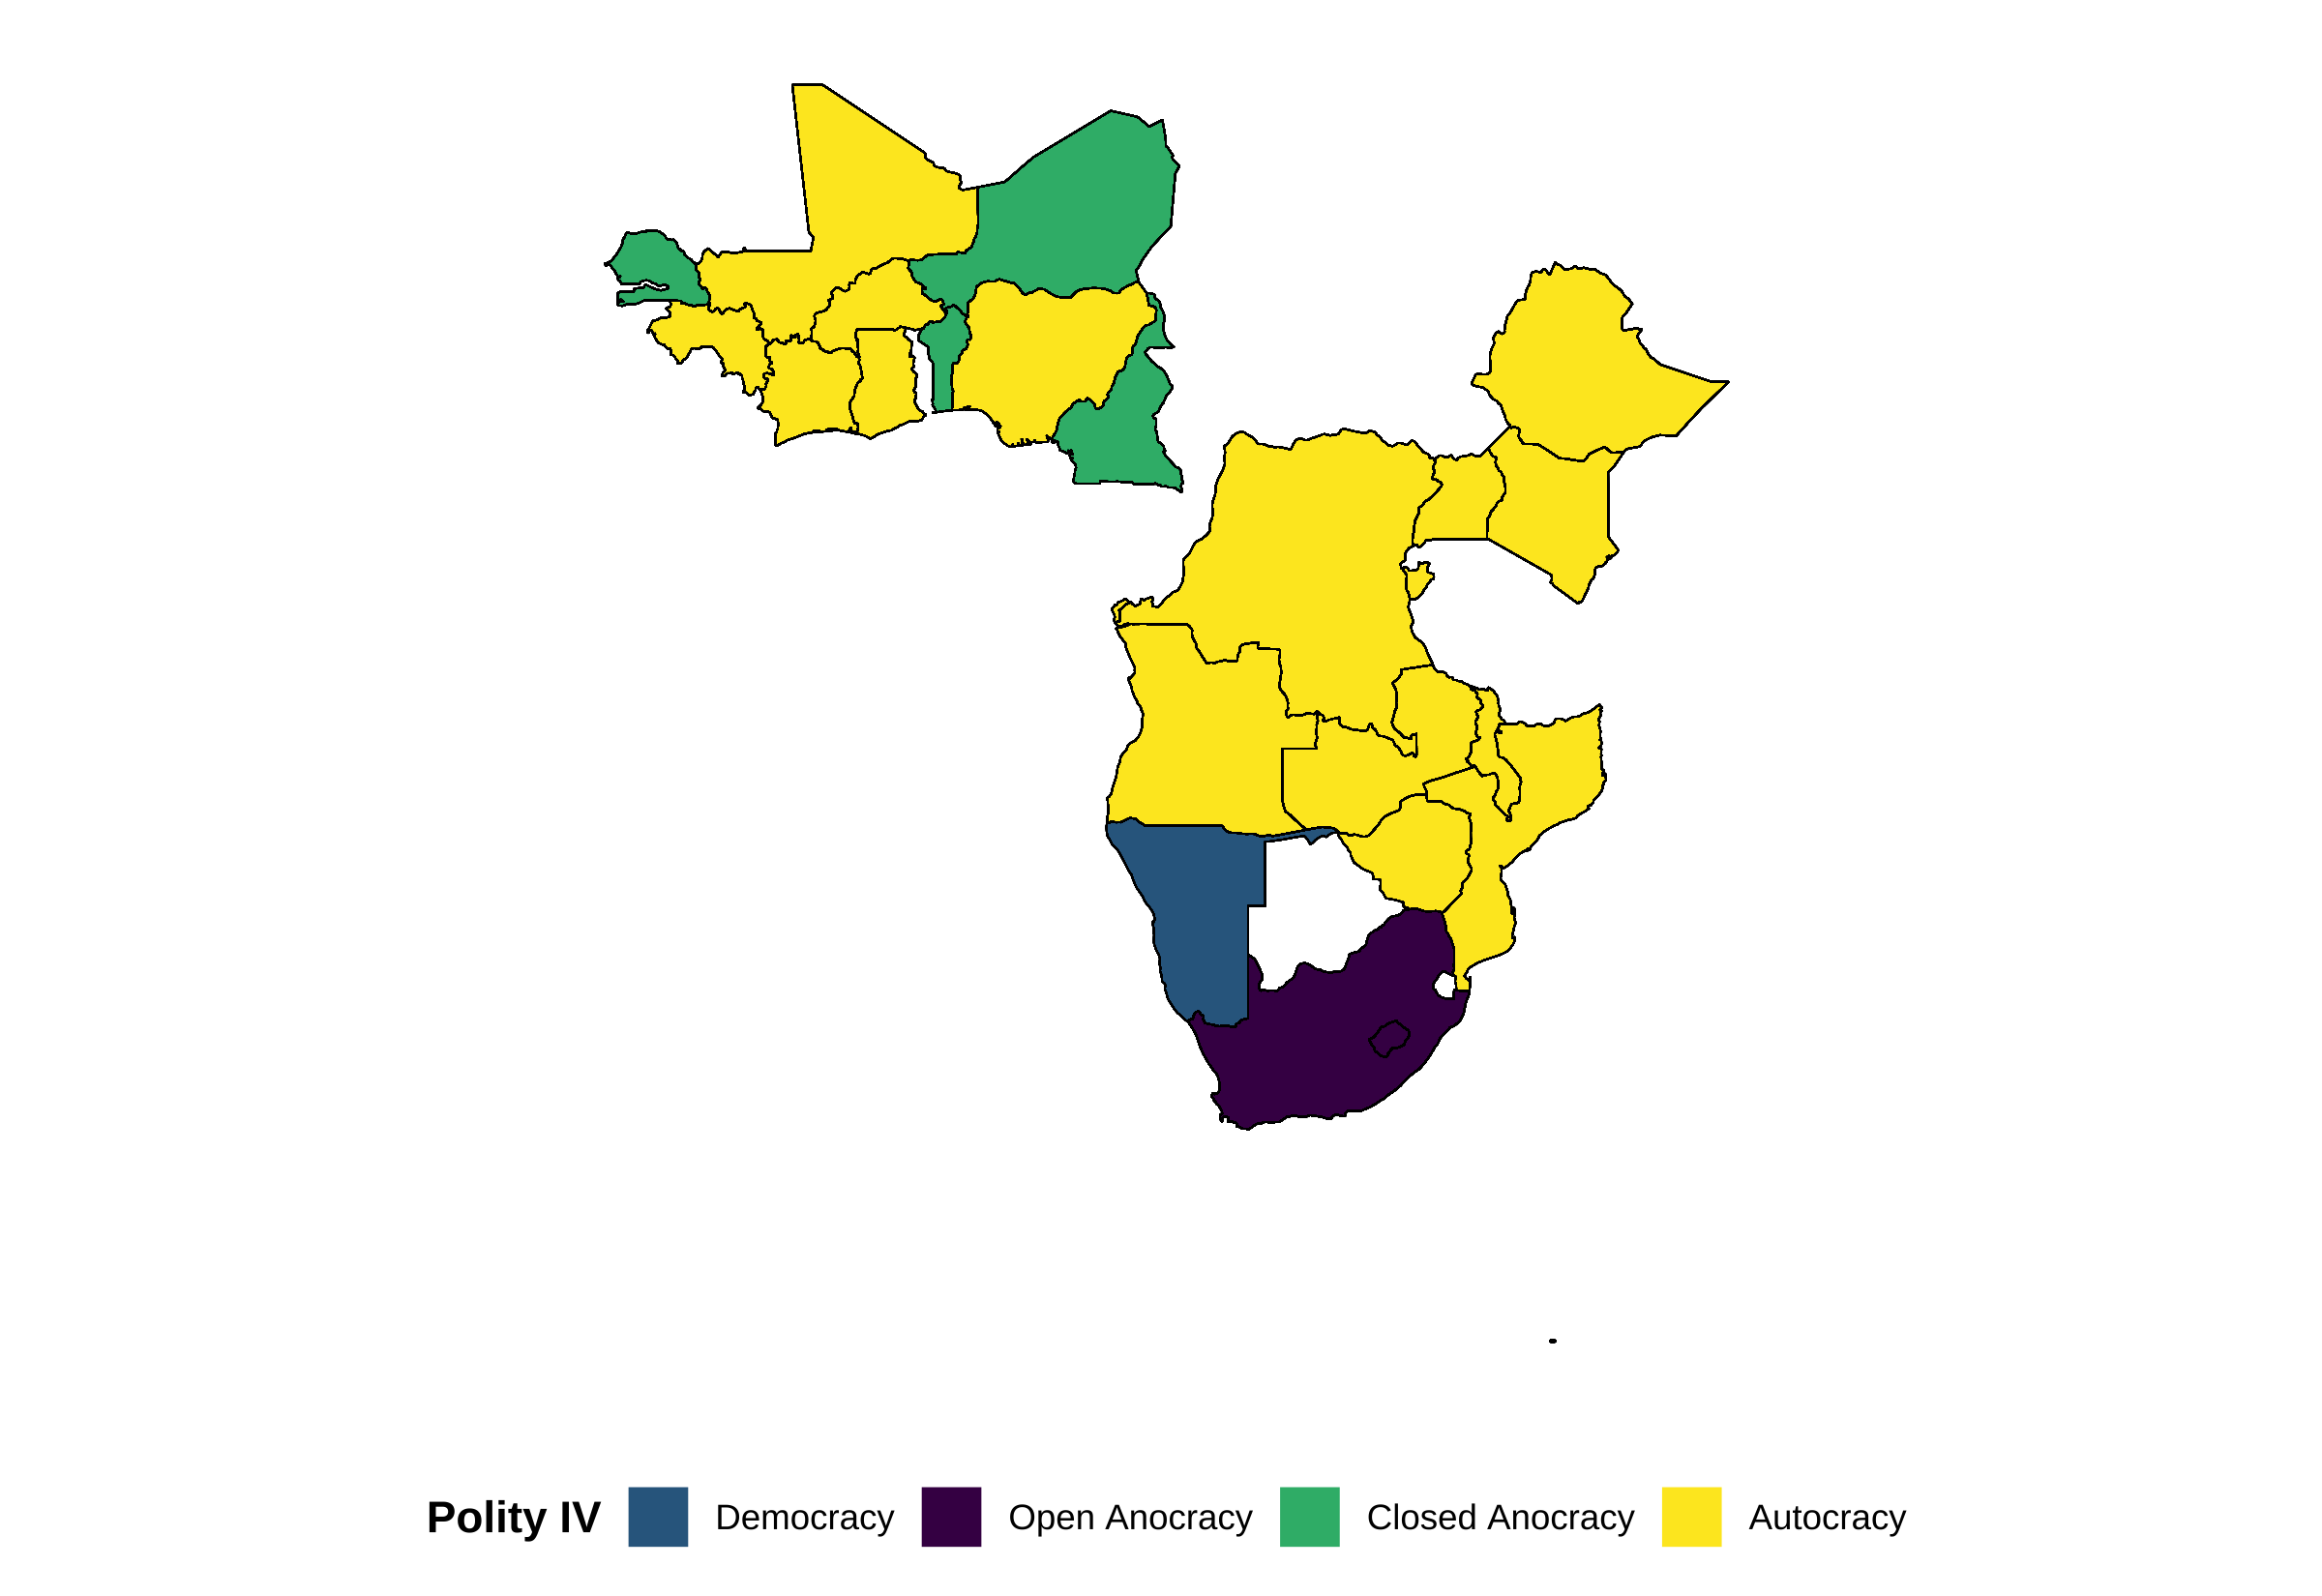
\includegraphics[width=.9\linewidth]{figure/1990.png}
\label{fig1990}
\end{subfigure}
% Fourth
\begin{subfigure}{.48\textwidth}
\centering
\caption{Polity Scores in 1995.}
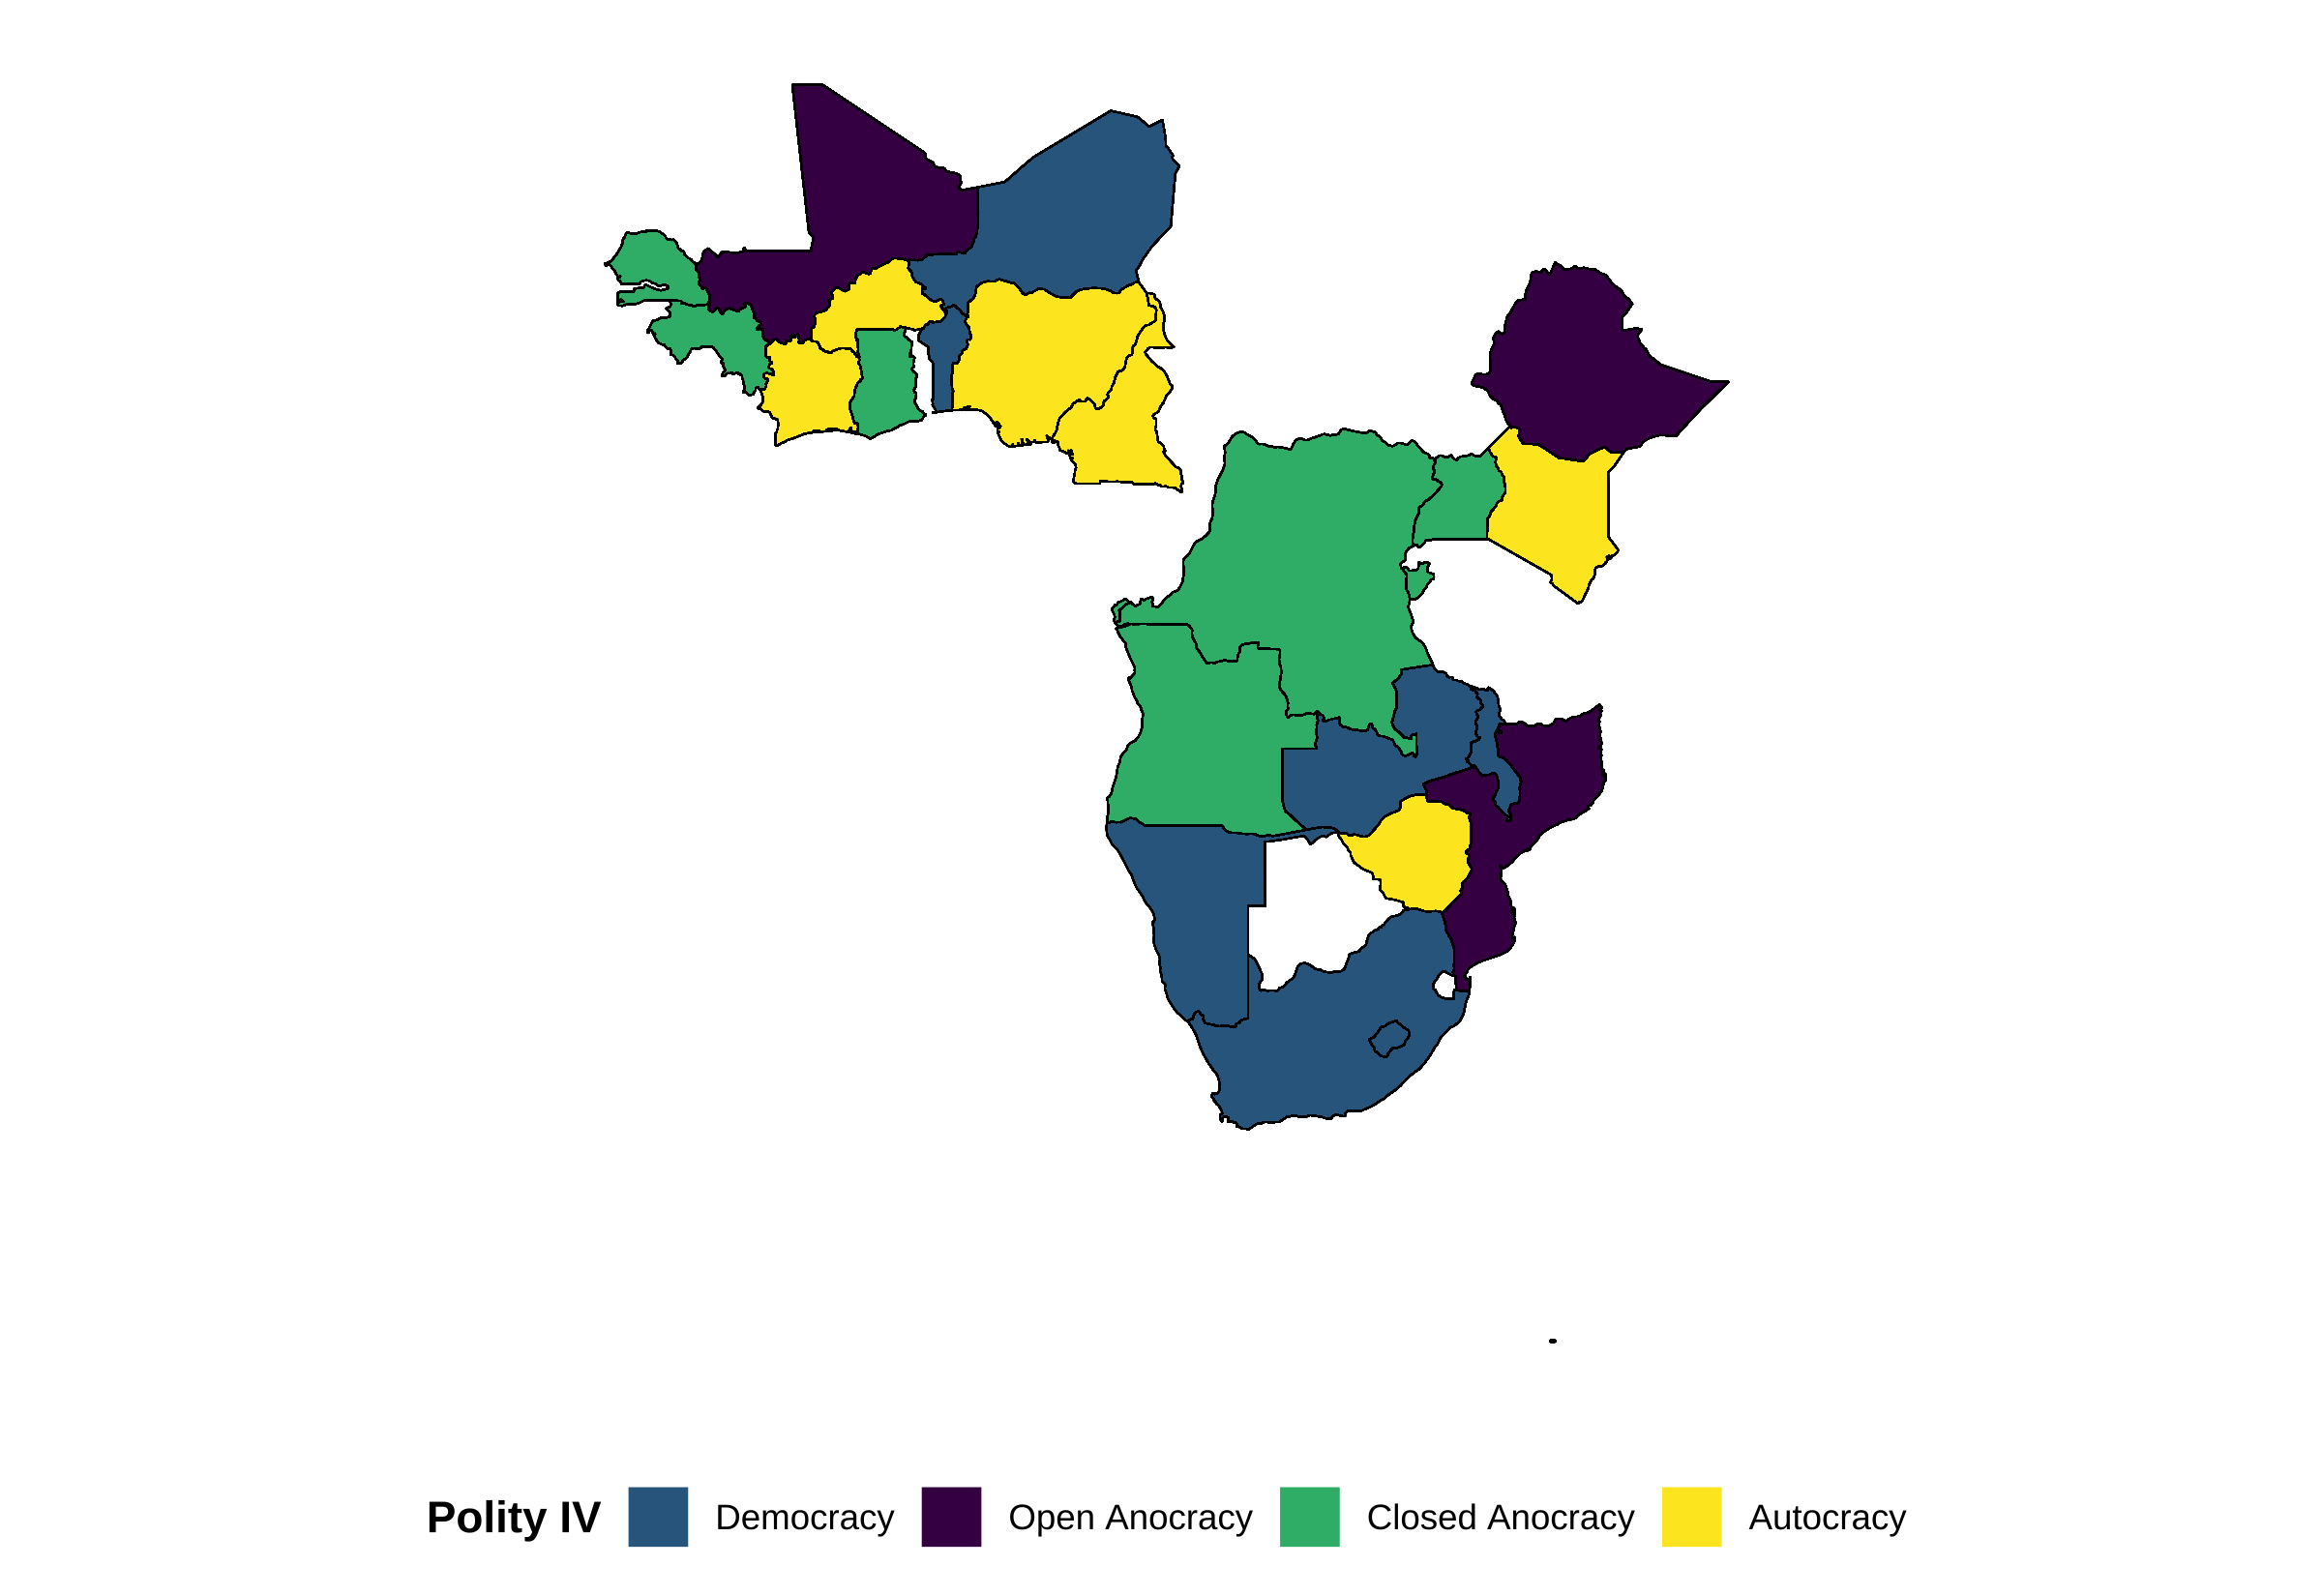
\includegraphics[width=.9\linewidth]{figure/1995.png}
\label{fig1995}
\end{subfigure}
%Fifth
\begin{subfigure}{.9\textwidth}
\centering
\caption{Polity Scores in 2000}
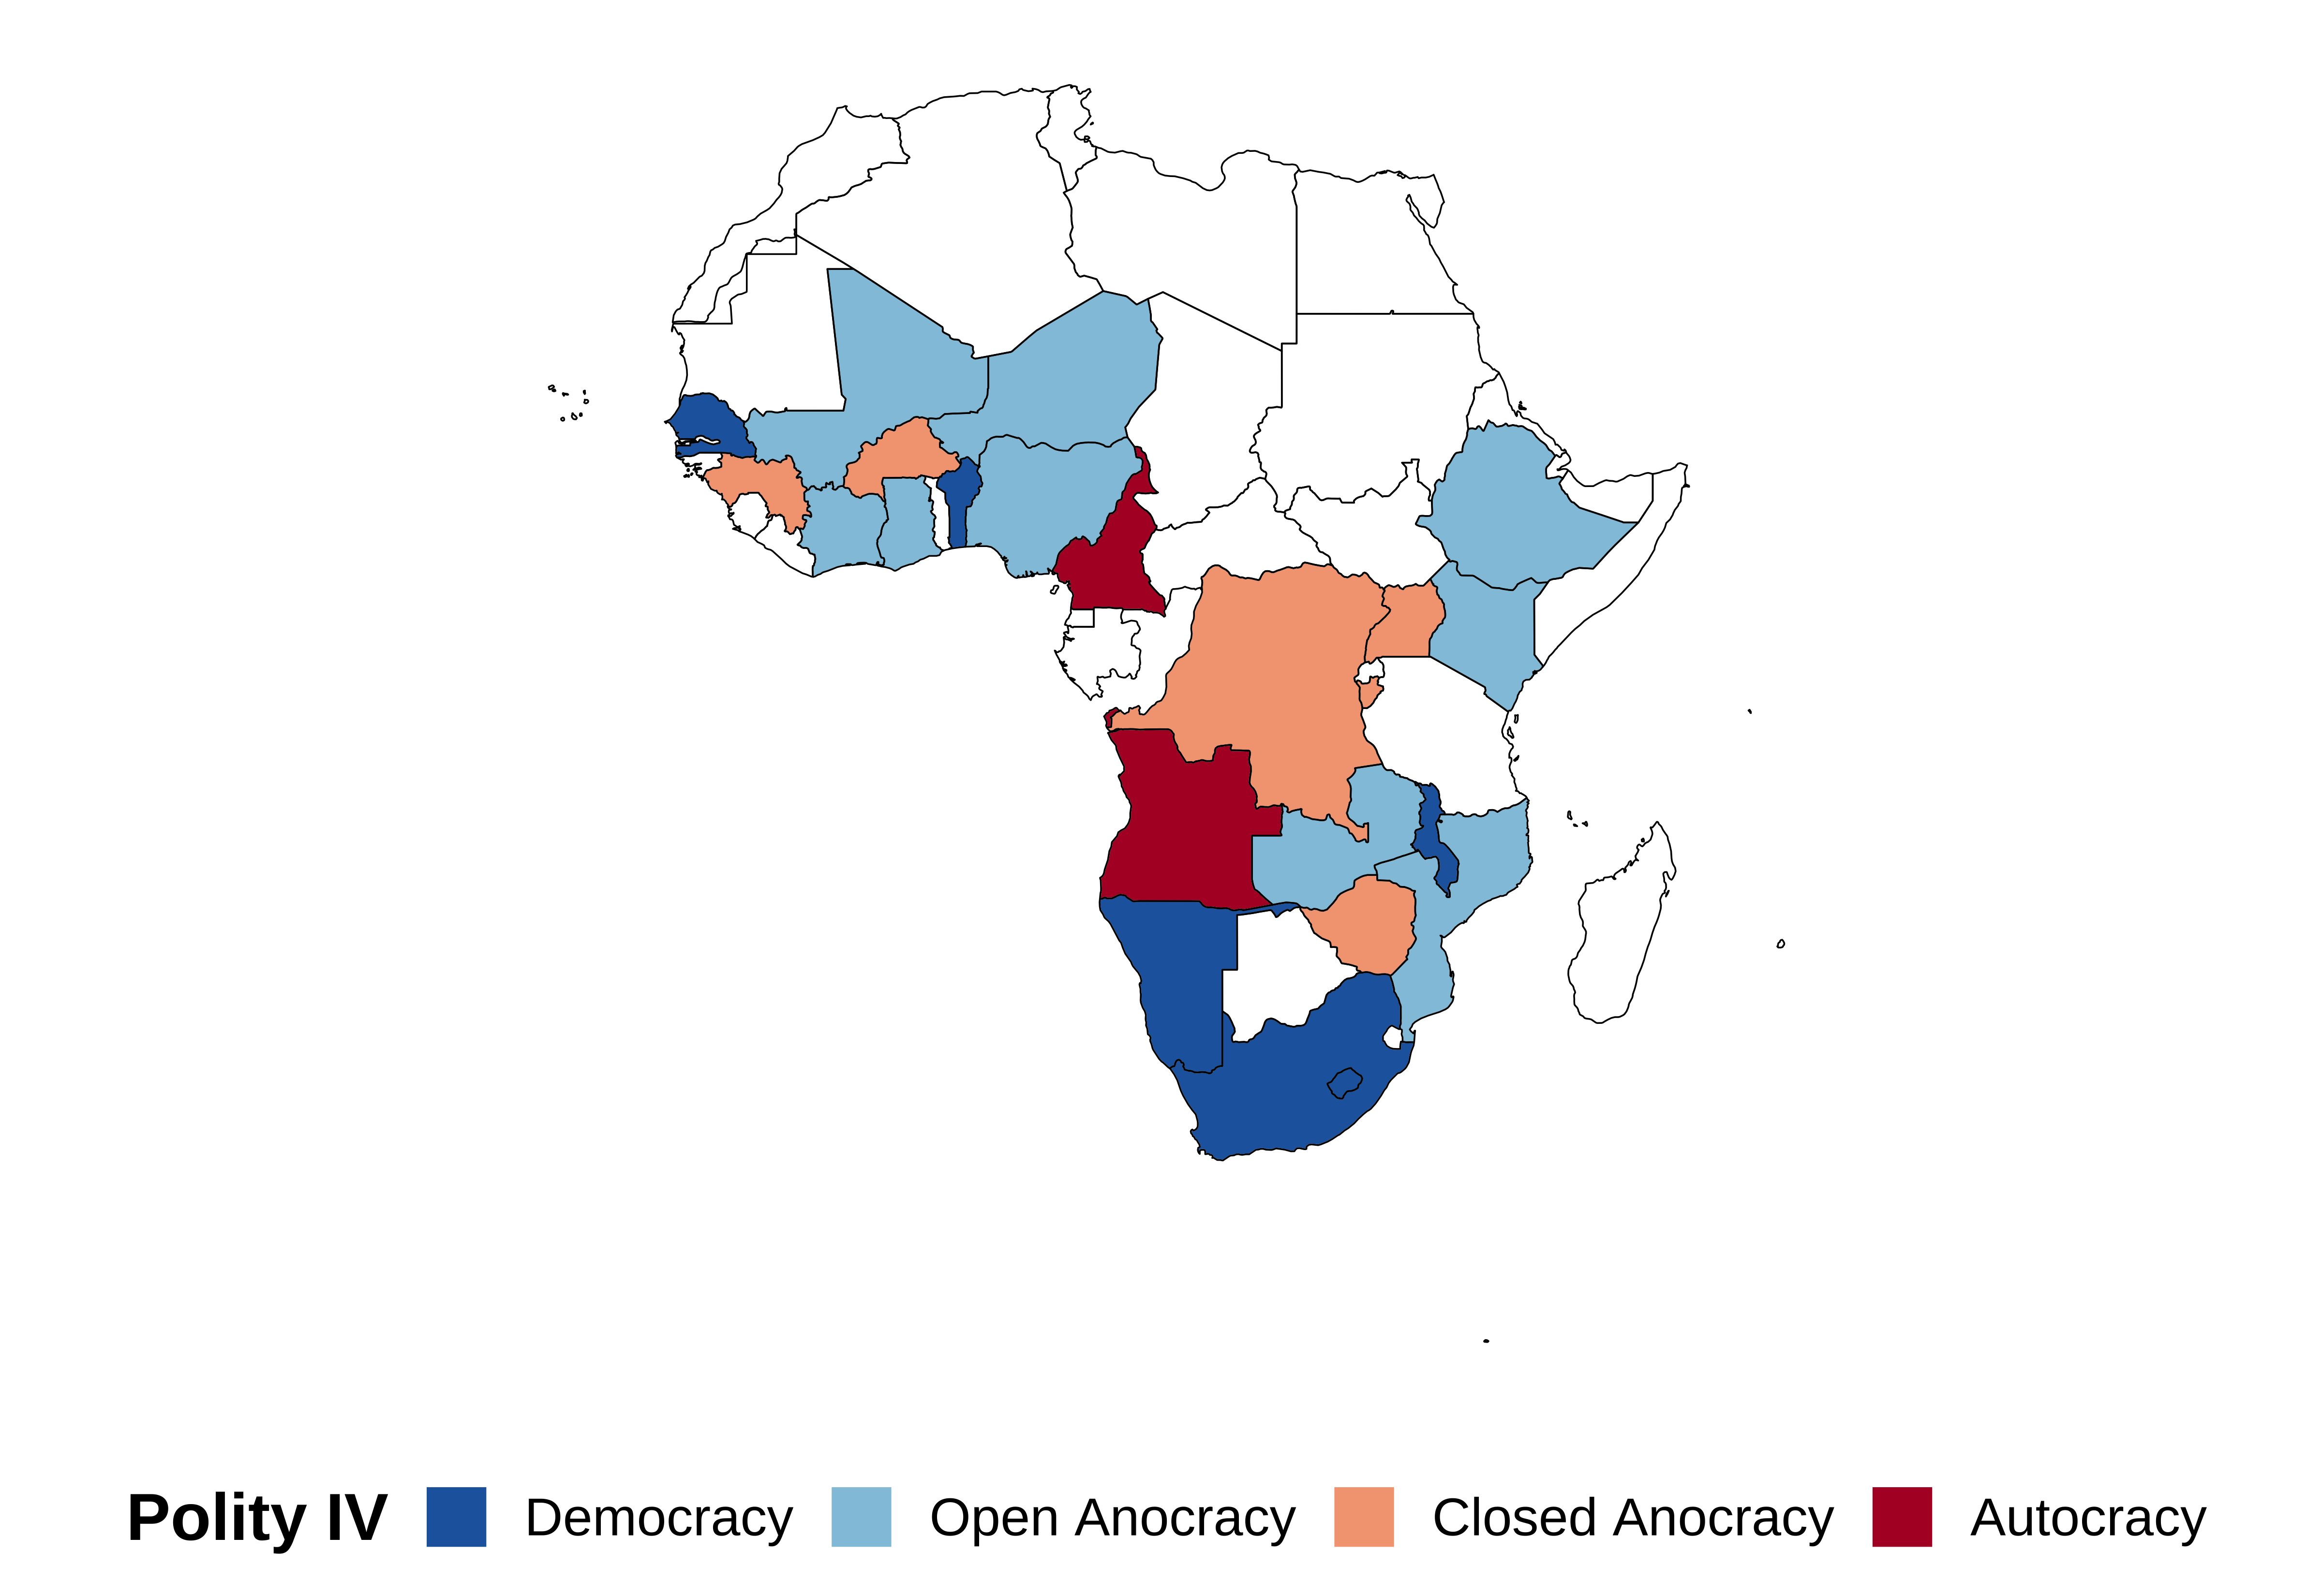
\includegraphics[width=.5\linewidth]{figure/2000.png}
\label{fig2000}
\end{subfigure}

\note{In this figure, I present the changes in Polity IV scores in the countries I am studying from 1980 to 2000. Notice Africa's democratization.}

\end{figure}

\subsection{Leaders, their ruling period and ethnicity}
To construct a variable for co-ethnicity, I had to know the ethnic group of every leader in my sample. Consequently, I rely on Archigos, a data set that records the name of every leader of a country since its independence \citep{goemans2006archigos}. I also use the data from \citet{fearon2007ethnic} to construct a data set on the ethnicity of leaders around the world from 1945 to 1999. I supplment \citet{fearon2007ethnic} the data to include more years, and consequently, more leaders.


\section{The Empirical Model}\label{sec4}
\subsection{Ethnic Favoritism in Africa.}
In this section, I will test for the existence of ethnic favoritism in Africa. Using the DHS data, I can investigate the existence of ethnic favoritism using a few outcomes of interest like education, wealth, electrification, access to drinking water and infant survival.

To estimate the average ethnic favoritism, I will run the following regression:

\begin{equation}\label{eqFR1}
\begin{split}
    Y_{iceta} &= \beta_{1}coethnic_{iceta}
    + \delta_{t} + \gamma_{ce} +\eta_{a}  + \varepsilon_{iceta}
\end{split}
\end{equation}

Where $Y_{iceta}$ is the outcome of interest of person $i$ in the country  $c$, of an ethnic group $e$ that was born at time $t$\footnote{In the cases when the outcomes are education, electrification, wealth and access to water $t$ is the time of the survey. In the case when the outcome is infant survival, $t$ is the year of birth.} and with age at the time of survey $a$. While $coethnic_{iceta}$ is a variable that indicates the co-ethnicity between person $i$ and the leader of a country at a given time. Under the specification I am using, co-ethnicity is a dummy variable that is equal to one if a person \textit{i} is co-ethnic with the leader of a country at a given time. I also used other specifications for co-ethnicity in which the co-ethnicity variable takes values between 0 and 1 to indicate the portion of time spent under a co-ethnic leader. The variables $\delta_{t}, \gamma_{ce}$ and $\eta_{a}$  are, respectively, vectors of time, country-specific ethnic group and age at the time of survey fixed effects.

Coefficient $\beta_{1}$ from equation \ref{eqFR1} estimates the differences in outcomes between co-ethnics and non-co-ethnics. If $\beta_{1} > 0$, then the ethnic kins of a president enjoy an advantage in outcome $Y$. If $\beta_{1} < 0$, the people that do not share the same ethnicity as their leader enjoy an advantage in outcome $Y$. Finally, when $\beta_{1} = 0$ there is no evidence that co-ethnics enjoy an advantage or disadvantage when compared to non-co-ethnics. 

For $\beta_{1}$ to be interpreted as ethnic favoritism, the differences in outcomes should be driven solely by a disproportional allocation of resources from a leader to their ethnic kins. The specification in equation \ref{eqFR1} helps disentangle and weed out some of the threats to the identification. I am compare the differences in outcomes of the different groups during periods when the president was from their groups to period when the president was not from their group. Thus, the helps separate the effect of having a co-ethnic as a president from other factors, like positive shocks to agriculture. Moreover, including survey year and ethnic group, fixed effects can produce an estimate that separates the effect of having a co-ethnic leader in power from group-specific and time-invariant characteristics.

Furthermore, as pointed out by \citet{kramon2013benefits}, the problem of stock \textit{versus} flow threaten identification. This problem is specifically severe when studying the effect of co-ethnicity on access to electricity and clean drinking water. Electrification and access to clean water can persist for a long time (stock). The fact that we can observe the different groups at a different point in time---using the different DHS waves--- I can compare if having a co-ethnic president did affect access to the two services. As for education and infant survival, we know when an infant was born---a health care service was provided--- and we know when a person received a year of primary education. Therefore, we can pin down the effect of co-ethnicity and make a stronger inference.

\subsection{Ethnic Favoritism and Democracy in Africa.}
The data I obtained allow me to construct a rich empirical model to investigate the existence of a differential and heterogeneous co-ethnic effect between countries that are more or less democratic. My specification also allows me to identify the effect of democracy within countries. I describe the regressions in equations \ref{eq1} and \ref{eq2}. Since I aim to study the effect of ethnic favoritism, I had to use the ethnicity variables provided by the DHS and the ethnic group of a leader from \citet{fearon2007ethnic} to create the co-ethnicity dummy variable. This variable is equal to one if person \textit{i} and the leader of the country they live in are from the same ethnic group. 

The regression equations I will use are given by:
\begin{equation}\label{eq1}
\begin{split}
   Y_{iceta} &= \beta_{1}coethnic_{iceta} + \beta_{2}DemocracyIndex_{ct} + \\
   & \beta_{3}coethnic_{iceta} \cdot DemocracyIndex_{ct}   + \delta_{t} + \gamma_{ce} +\eta_{a}  + \varepsilon_{iceta}
\end{split}
\end{equation}

\begin{equation}\label{eq2}
\begin{split}
    Y_{iceta} &= \beta_{1}coethnic_{iceta} + \beta_{2} I_{(5\leq Polity IV \leq 10)} + \beta_{3} I_{(-5\leq Polity IV \leq 5)} + \\
    &\beta_{4} I_{(5\leq Polity IV \leq 10)} \cdot  coethnic_{iceta} + \beta_{5} I_{(-5\leq Polity IV \leq 5)} \cdot  coethnic_{iceta} + \\
    &\delta_{t} + \gamma_{ce} +\eta_{a}  + \varepsilon_{iceta}
    \end{split}
\end{equation}

Where $Y_{iceta}$ is the outcome of interest for person $i$ in the country $c$, ethnic group $e$, at period $t$\footnote{In the cases when the outcomes are education, electrification, wealth and access to water $t$ is the time of the survey. In the case when the outcome is infant survival, $t$ is the year of birth.} and with age at the time of the survey $a$. $coethnic_{iceta}$ is the dummy variable for co-ethnicity and is equal to one of the observation $i$ is the same ethnicity as the leader at time $t$ in the country $c$. $DemocracyIndex_{ct}$ is the index for democracy. Variables $I_{(5\leq Polity IV \leq 10)}$, and $I_{(-5\leq Polity IV \leq 5)}$ are indicator variables of democratic bins that respectively represent democracies, and anocracies. $I_{(-10\leq Polity IV \leq -5)}$ is the omitted dictatorship group. The variables $\delta_{t}, \gamma_{ce}$ and $\eta_{a}$  are, respectively, vectors of time, country-specific ethnic group and age at the time of survey fixed effects.

We are interested in variables $\beta_{3}$ from equation \ref{eq1} and $\beta_{5}$, and $\beta_{6}$ from \ref{eq2}. $\beta_{3}$ and $\beta_{5}$, and $\beta_{6}$ estimate the differences and relationships of ethnic favoritism in democratic/anocratic and autocratic countries on the outcomes of interest.

\section{Results and Discussion}\label{sec5}

In this section, I will introduce the results of estimating my empirical models. First, I investigate the existence of ethnic favoritism on schooling, electrification, access to clean drinking water, wealth and infant survival. I find evidence of ethnic favoritism on infant survival and access to clean drinking water (equation \ref{eqFR1}). Second, I include a measure of democracy and investigate the effect of democracy on ethnic favoritism on the outcomes of interest. The interaction between democracy and co-ethnicity is statistically significant when studying their effect on electrification and access to clean drinking water (equation \ref{eq2}).

I find evidence of ethnic favoritism on infant survival and access to clean drinking water. When I introduce a measure of democracy, I find a statistically significant effect of the interaction between democracy and co-ethnicity on electrification and access to clean drinking water. A child whose mother is a co-ethnic of the leader in power two years before their birth is 1.3 percentage points more likely to survive their first year after birth.  A person who was of the same ethnicity as the leader two years prior to the survey is more likely to have access to clean drinking water than a non-co-ethnic person. Putting the ethnic favoritism on infant survival in perspective, 87.5\% of non-co-ethnic children in the sample survive the first year of life. Consequently, ethnic kins would, on average, have a survival rate of 88.8\%. However, when comparing co-ethnic and non-co-ethnics in democracies or anocracies and autocracies, I find evidence of ethnic favoritism on electrification and access to clean drinking water in anocracies and democracies as well as education in anocracies.

\subsection{Existence of Ethnic Favoritism} \label{subsec1}
I look into the existence of ethnic favoritism on primary school completion, electrification, access to clean drinking water, wealth and infant survival.\footnote{The primary school completion is a dummy variable that is equal to 1 if a person completed primary school and zero otherwise. The co-ethnic variable for education as an outcome is equal to the total years between the ages of seven and thirteen that a person lived under the rule of a co-ethnic leader divided by seven. For electrification and access to water, the co-ethnic variable is equal to one of the leaders two years before the interview date was a co-ethnic. For wealth, the co-ethnic variable is equal to the total years a person spent under the rule of a co-ethnic leader in the four years before the interview was conducted divided by four. For infant mortality, the co-ethnic variable is a dummy that is equal to one of the presidents who was of the same ethnicity as the mother the year the child was born. The infant mortality variable was constructed following \citet{kudamatsu2009ethnic, kudamatsu2012has}.} I report the results in table \ref{tab:eth} and figure \ref{fig:coeet}. These results are the estimates of equation \ref{eqFR1}. 

\begin{table}[!h]

\caption{Ethnic favoritism results \label{tab:eth}}
\centering
\resizebox{\linewidth}{!}{
\begin{threeparttable}
\begin{tabular}[t]{lccccc}
\toprule
  & \specialcell{(1) \\ Schooling} & \specialcell{(2) \\ Infant Survival} & \specialcell{(3) \\ Wealth} & \specialcell{(4) \\ Electrification} & \specialcell{(5) \\ Clean Water}\\
\midrule
Coethnic & \num{-0.038} & \num{0.005} & \num{0.001} & \num{0.042}*** & \num{-0.028}\\
 & (\num{0.024}) & (\num{0.004}) & (\num{0.023}) & (\num{0.016}) & (\num{0.032})\\
\midrule
Mean & \num{0.649} & \num{0.905} & \num{0.275} & \num{0.351} & \num{0.216}\\
N & \num{1146305} & \num{2516753} & \num{756737} & \num{822353} & \num{822353}\\
\bottomrule
\multicolumn{6}{l}{\rule{0pt}{1em}* p $<$ 0.1, ** p $<$ 0.05, *** p $<$ 0.01}\\
\end{tabular}
\begin{tablenotes}
\item[1] \footnotesize{In this table, I am reporting the estimates of equation \ref{eqFR1}. 
                      I present the results of the effect of ethnic favoritism on primary school completions 
                      in column 1, infant survival in column 2, top wealth quintile in column 3, electrification in 
                      column 4 and access to clean drinking water in column 4. Primary school completion is a 
                      dummy variable that is equal to one if a person completed primary school and zero otherwise. 
                      Infant survival is a dummy variable that is equal to one if an infant survived the first 12 
                      months of life. Wealth is a dummy variable that is equal to one if a person belongs to the top 
                      wealth quintile. Electrification is a dummy variable that is equal to one if a household 
                      has electricity. Finally, access to clean drinking water is a dummy variable that is equal to one if a household 
                      has access to clean piped drinking water.}
\item[2] \footnotesize{Standard errors are clustered on country specific ethnic groups. All results include ethnic group, time and age fixed effects.}
\end{tablenotes}
\end{threeparttable}}
\end{table}


In table \ref{tab:eth},  I estimate the average effect of having a co-ethnic leader on primary school completion (column 1), infant survival (column 2), wealth quintile (column 3), electrification (column 4) and access to clean drinking water (column 5). A respondent that spent all of her primary school under the rule of a co-ethnic leader was $3.8$ percentage points less likely to finish primary school, but the result was statistically insignificant (table \ref{tab:eth} column 1). As for children's health (table \ref{tab:eth} column 2), a child whose mother was of the same ethnic group as the president two years before birth was as likely to survive the first 12 months of their life. A person that lived under the rule of a co-ethnic leader in the four years before the survey is as likely to be in a higher wealth quintile (table \ref{tab:eth} column 3). Finally, a respondent that had a co-ethnic leader two years before the survey was conducted is more than 4.2 percentage points more likely to have electricity and as likely to have access to clean drinking water (table \ref{tab:eth} columns 4 and 5). To the exception of the effect of co-ethnicity on electrification, none of the other results were statistically significant. The point estimate of the effect of ethnic favoritism on primary school completion is large but insignificant. The confidence interval, however, includes mostly negative values. Ranging from $-8.55$  to around $0.88$ percentage points. To put this into perspective, 65\% of the sample completed primary school. Meaning that, on average, 67.1-80.9\% of co-ethnics finished primary school while 75.56-80.08\% of non-co-ethnics finished primary school.

\begin{figure}[!htb]
%Third
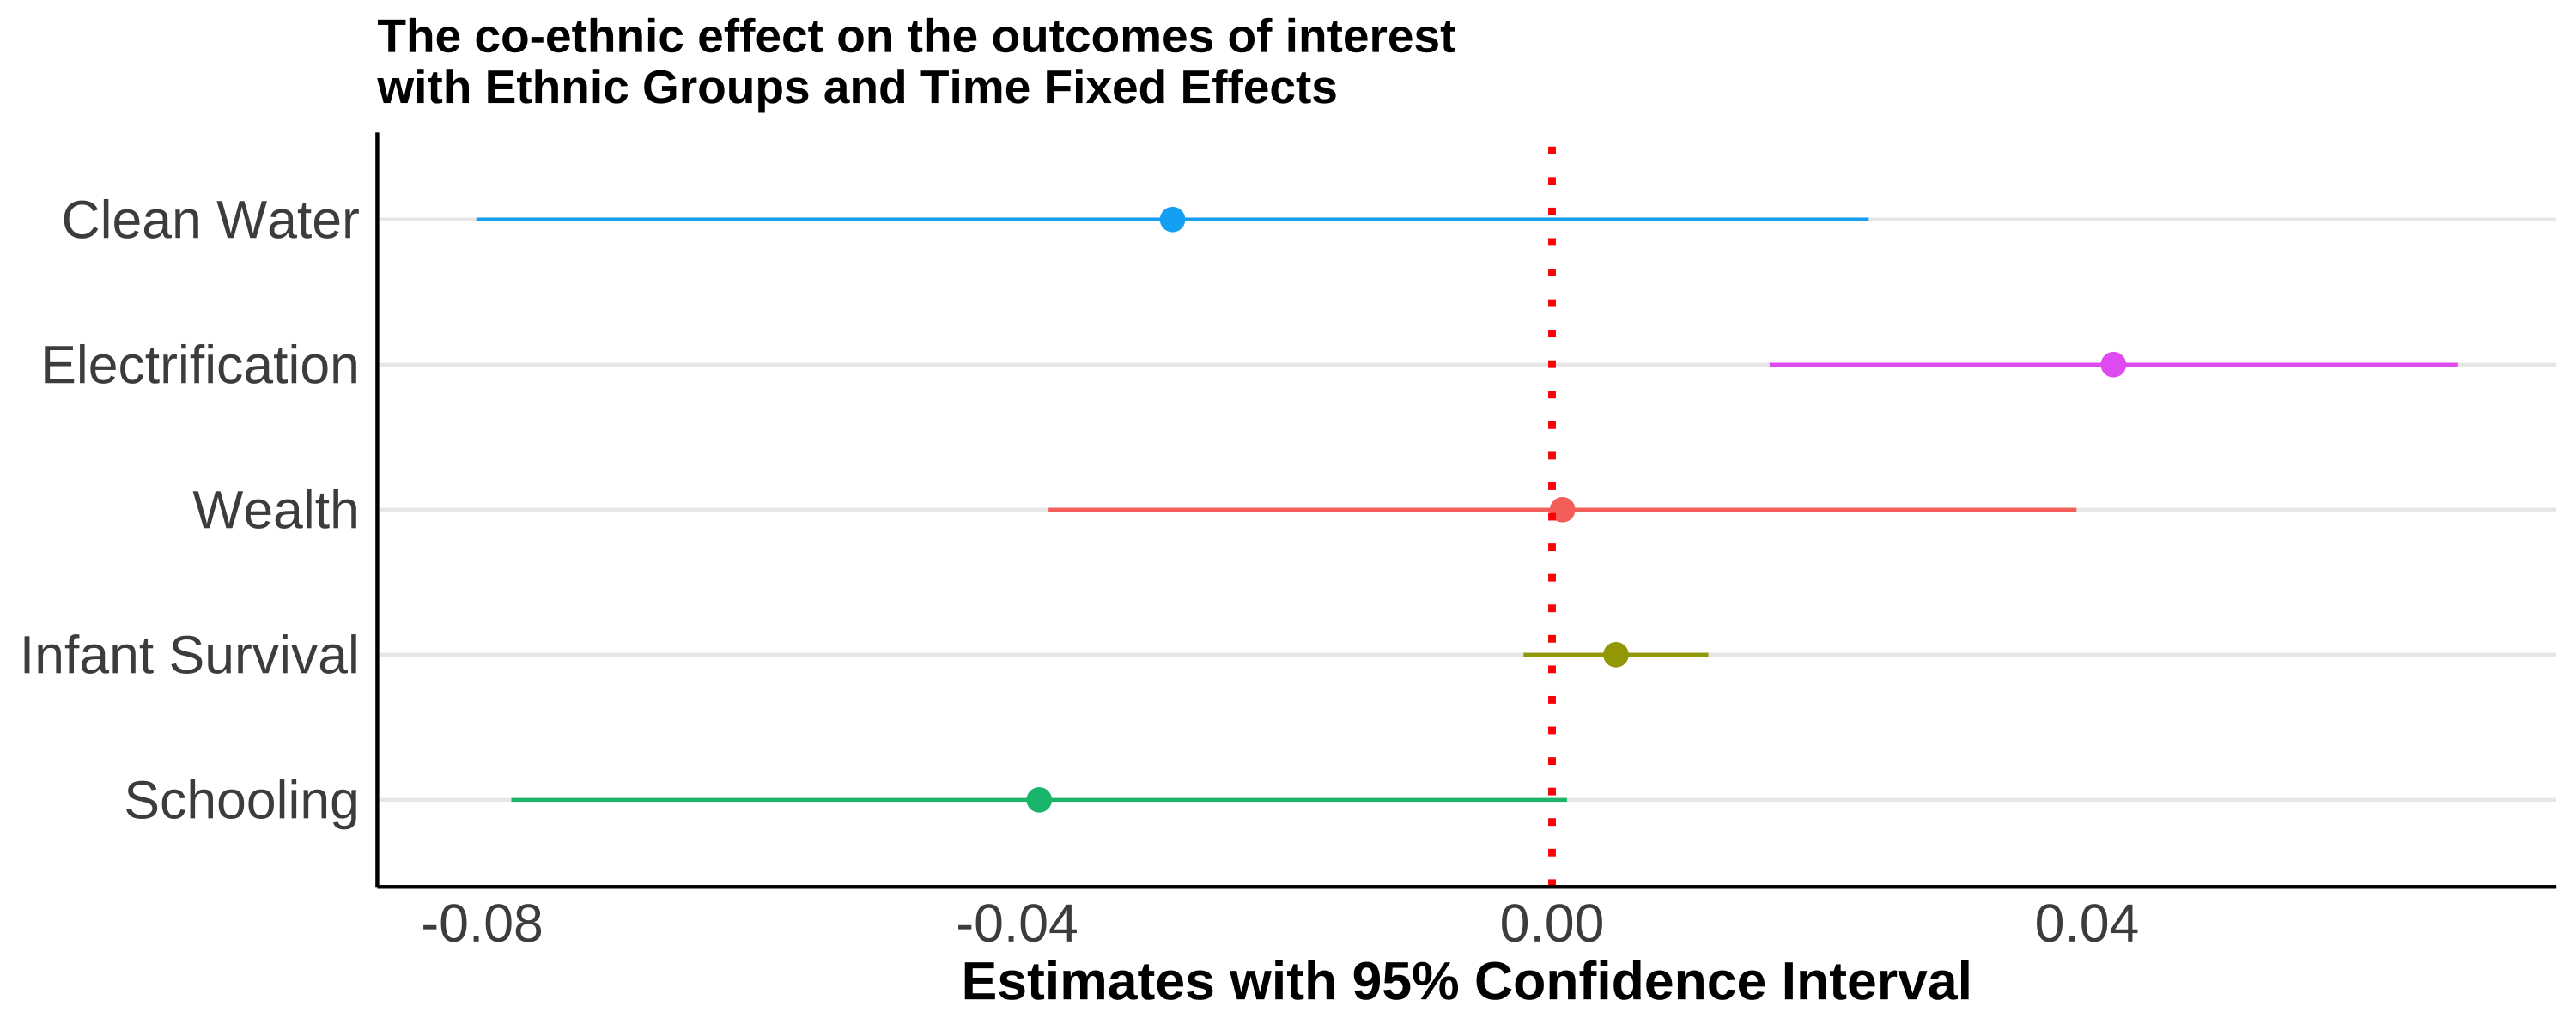
\includegraphics[width=.9\linewidth]{figure/coeth_ethFE.png}
\caption{Effect of co-ethnicity on outcomes of interest with ethnic group and time fixed effects.}
\label{fig:coeet}
\note{In this figure, I present the estimates of the co-ethnicity variable on primary school completion, infant survival, wealth, electrification and access to clean drinking water. The bands represent the 90\% confidence interval and the standard errors are clustered on ethnic groups. All estimates include ethnic group, time and age fixed effects.}
\end{figure}

% These results fit into the empirical results of \citet{kramon2013benefits} and the theoretical work of \citet{francois2015power}. In \citet{kramon2013benefits}, the authors found inconclusive evidence on the existence of ethnic favoritism. \citet{kramon2013benefits} did not find any evidence of systematic favoritism in one area across the six countries they analyzed. Favoritism was country-dependent. For example, they found no evidence of ethnic favoritism on education in Benin and Zambia. They also found that there is ethnic favoritism in education in Kenya and Malawi and ethnic disadvantage in Senegal and Mali. While \citet{francois2015power} showed that Africa is more ethnically representative than Western democracies. Consequently, the empirical results of this paper fit with the theory. Leader aims to stay in power. They appoint cabinet members of many ethnic groups hoping that these cabinet members will share the wealth with their ethnic groups. Therefore, they can maximize their time in power by preventing coups and revolutions. 

% \begin{figure}[!htb]
% \label{fig:grps}
% \centering
% \begin{subfigure}{.48\textwidth}
% \centering
% 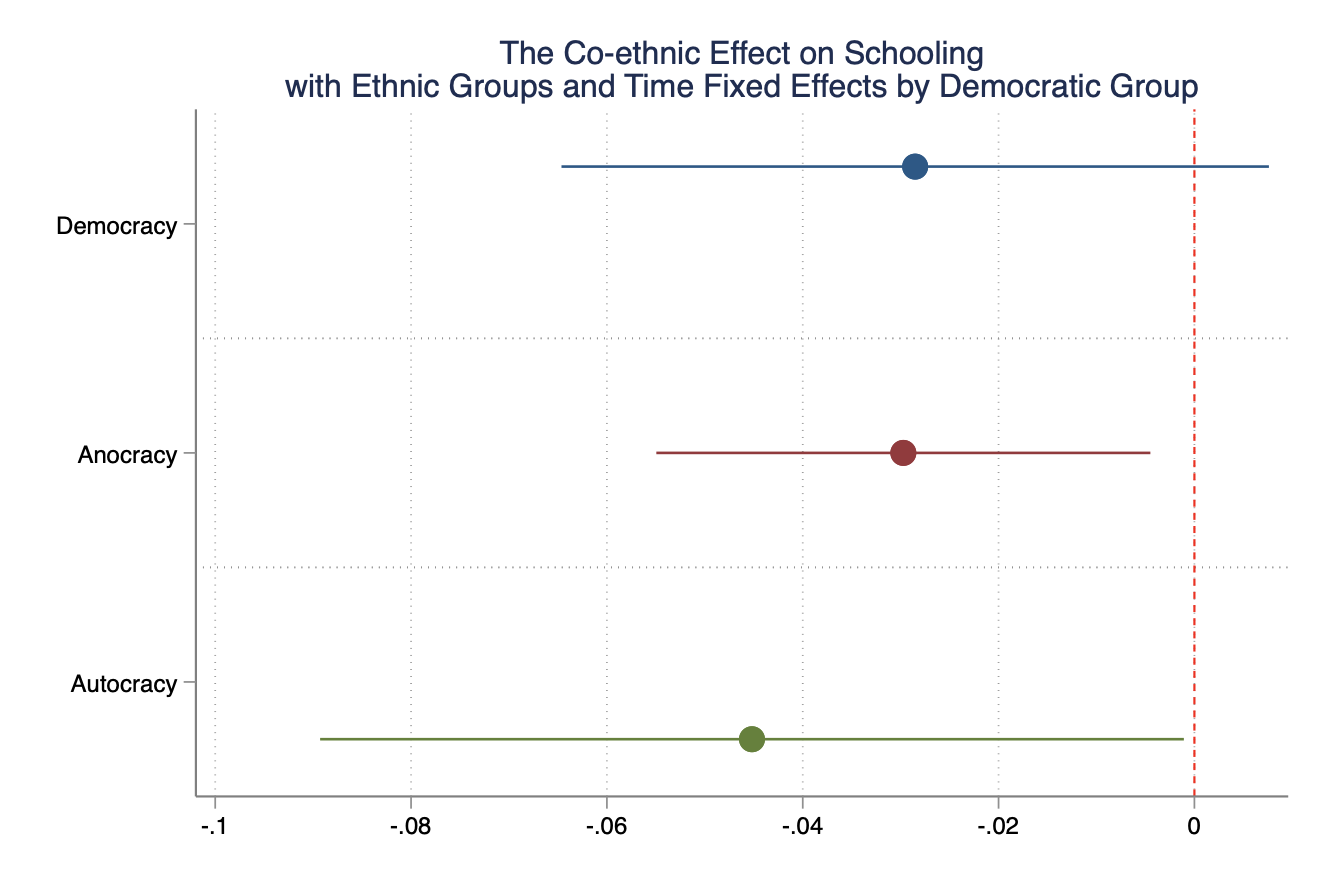
\includegraphics[width=.9\linewidth]{coeth_byGroups1.png}
% \caption{Effect of Ethnic Favoritism on Schooling, by Polity Groups.}
% \label{ethdemgrp1}
% \end{subfigure}
% \centering
% %Second graph
% \begin{subfigure}{.48\textwidth}
% \centering
% 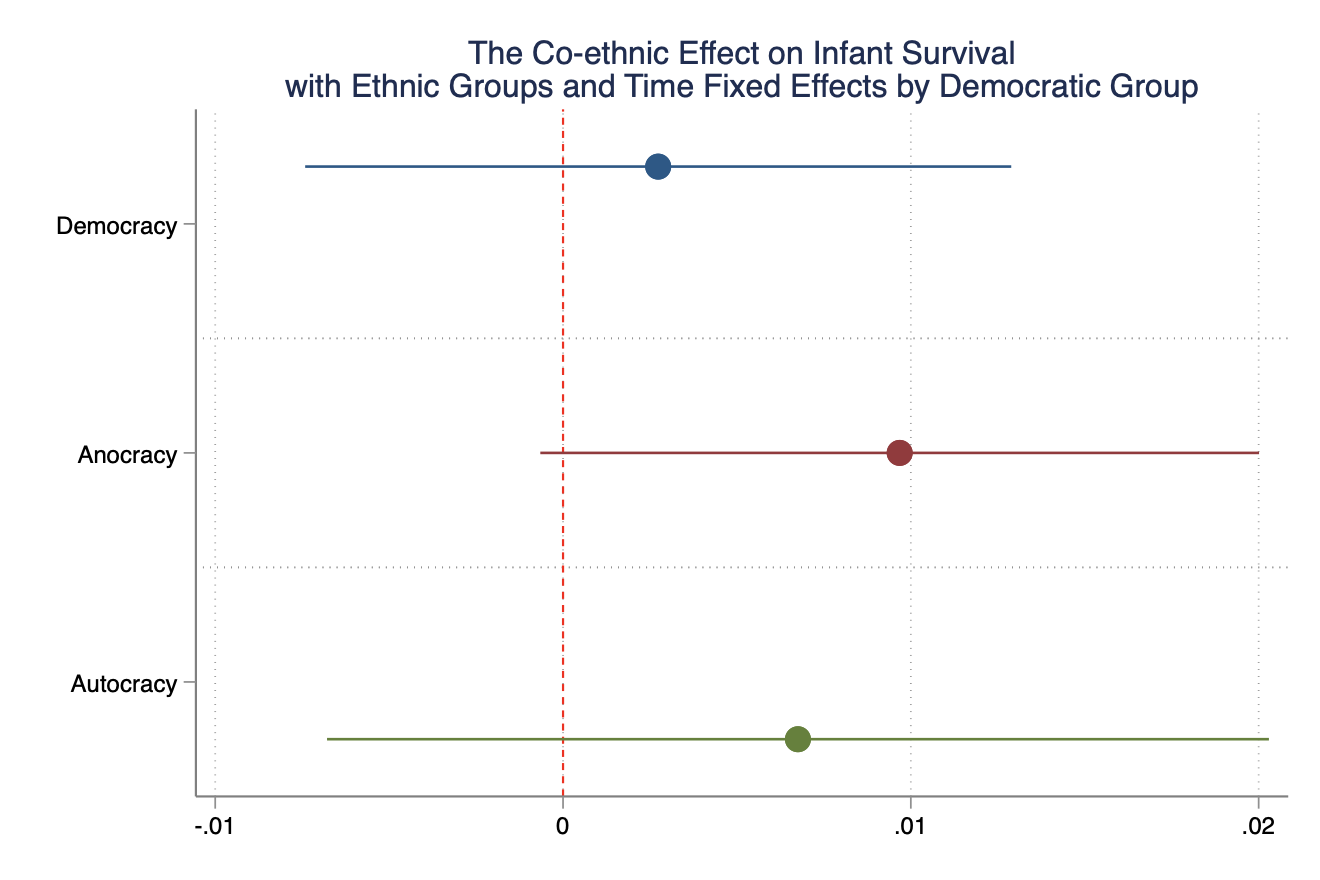
\includegraphics[width=.9\linewidth]{coeth_byGroups2.png}
% \caption{Effect of Ethnic Favoritism on Infant Survival, by Polity Groups.}
% \label{ethdemgrp2}
% \end{subfigure}
% %Third
% \begin{subfigure}{.48\textwidth}
% \centering
% 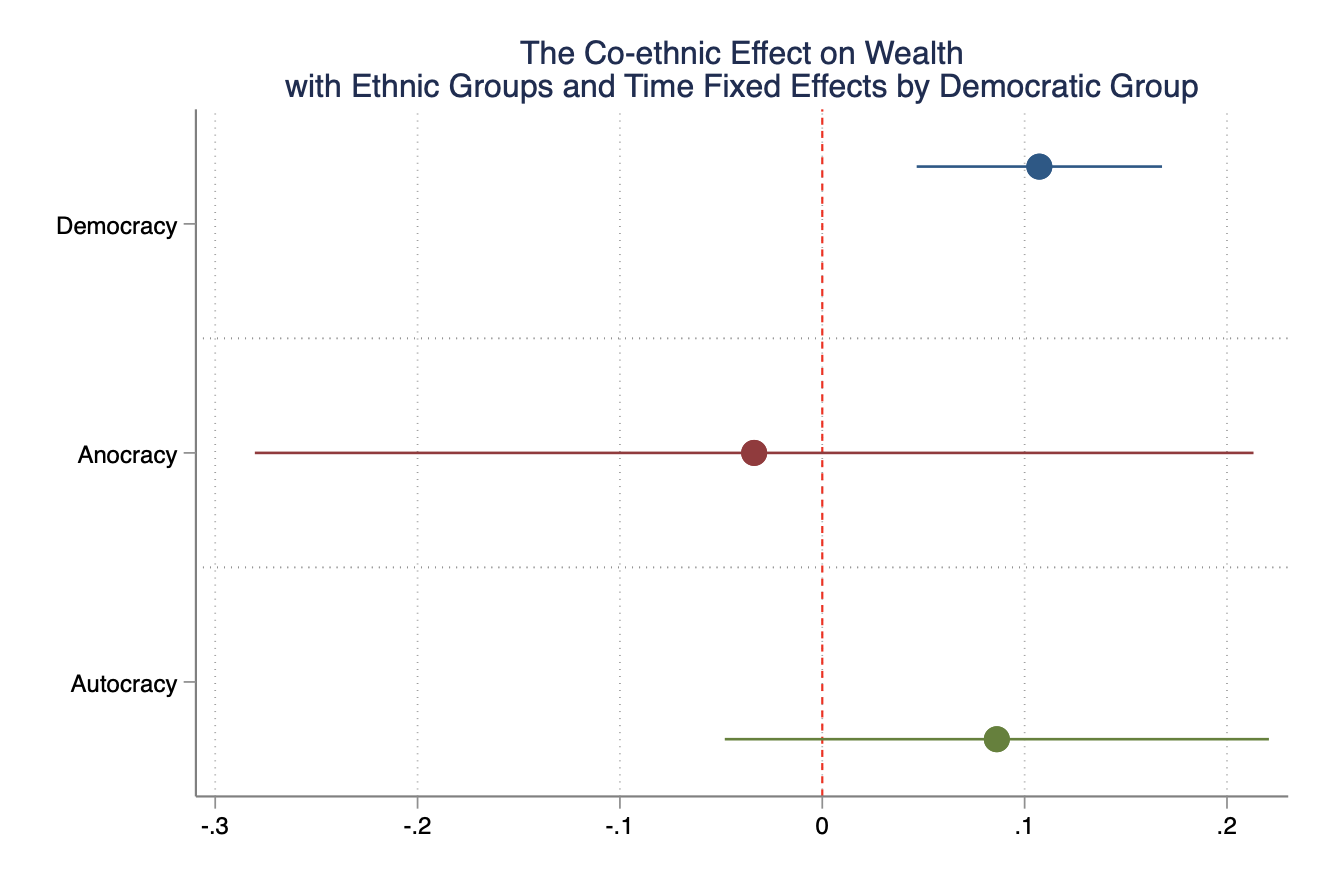
\includegraphics[width=.9\linewidth]{coeth_byGroups3.png}
% \caption{Effect of Ethnic Favoritism on Wealth, by Polity Groups.}
% \label{ethdemgrp3}
% \end{subfigure}
% % Fourth
% \begin{subfigure}{.48\textwidth}
% \centering
% 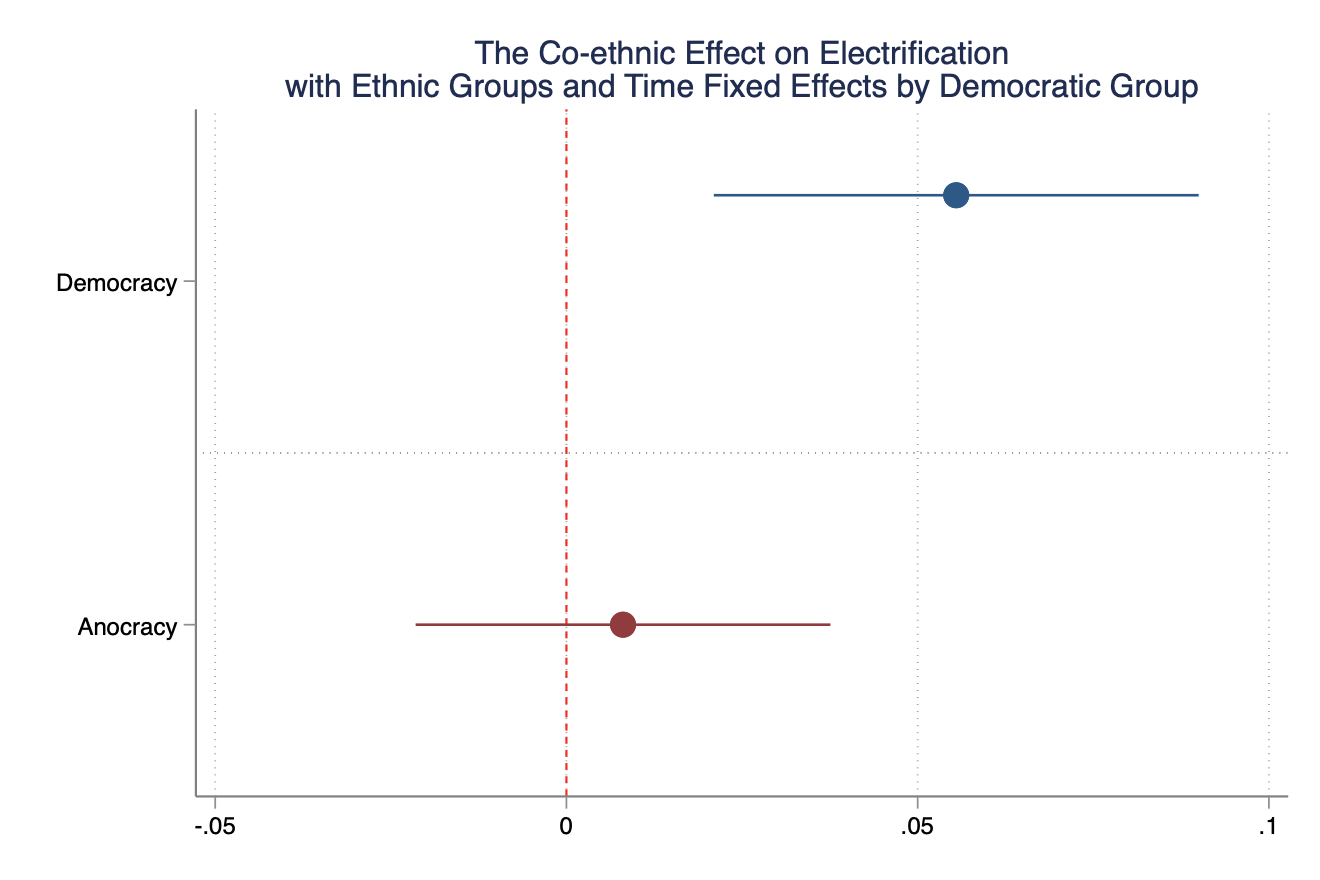
\includegraphics[width=.9\linewidth]{coeth_byGroups4.png}
% \caption{Effect of Ethnic Favoritism on Electrification, by Polity Groups.}
% \label{ethdemgrp4}\end{subfigure}
% %Fifth
% \begin{subfigure}{.9\textwidth}
% \centering
% 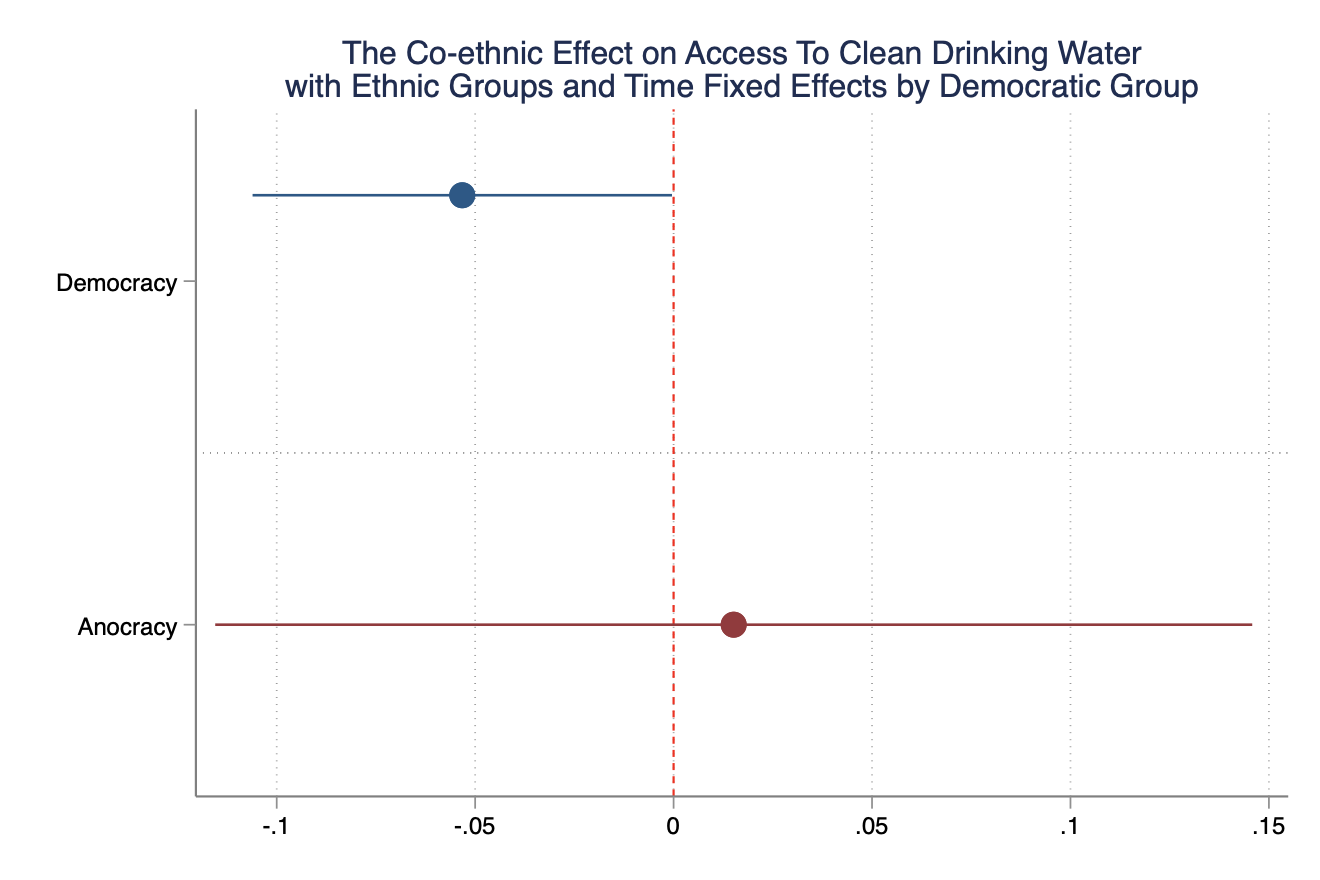
\includegraphics[width=.5\linewidth]{coeth_byGroups5.png}
% \caption{Effect of Ethnic Favoritism on Clean Drinking Water, by Polity Groups.}
% \label{ethdemgrp5}\end{subfigure}
% \caption{Effect of Ethnic Favoritism on Variables of Interest, by Polity Groups}
% \label{fig:demgrpseth}
% \note{In this figure, I present the estimates of the co-ethnicity variable on primary school completion, infant survival, wealth, electrification and access to clean drinking water by Polity IV groups. The bands represent the 90\% confidence interval and the standard errors are clustered on ethnic groups. All estimates include ethnic group, time and age fixed effects.}
% \end{figure}

%When studying the effect of ethnic favoritism on primary school completion, I generated a dummy variable using the information provided by the DHS on education. The primary school completion variable is a dummy variable that is equal to one if a person completed primary school and zero otherwise. The analysis indicates that coethnics do not benefit from having ethnic kin as a leader. A person living under the rule of a coethnic leader is 3.91\% less likely to complete primary school compared to a non-co-ethnic person. 
%
%Moreover, it appears that coethnicity does not affect infant mortality. I took advantage of the DHS's birth recode. I found no evidence supporting the existence of ethnic favoritism when it comes to infant mortality. A child that is co-ethnic with a leader on the year of birth has the same likelihood of dying in the first 12 months of her life as a non-coethnic.
%
%I test the existence of ethnic favoritism on wealth. The DHS creates a wealth variable that is the product of standardized z-scores and wealth indicators. The DHS defines the wealth index as:
%\begin{quote}
%The wealth index is a composite measure of a household's cumulative
%living standard. The wealth index is calculated using easy-to-use data 
%on a household's ownership of selected assets, such as televisions and bicycles; materials used for housing construction; and types of water access and sanitation facilities.
%
%Generated with a statistical procedure known as principal components analysis, the wealth index places individual households on a continuous scale of relative wealth. DHS separates all interviewed households into five quintiles of wealth.
%\end{quote}
%
%The results of the regressions I ran on wealth are in table \ref{tab:eth}. Coethnics with the country's leader is more likely to belong to higher wealth quintiles than non-coethnics. Thus, coethnics accumulated more wealth during the tenure of their leader.
%
%
%I also used the electrification information that the DHS collects to search for ethnic favoritism in this area. I found statistically significant results that indicate the existence of ethnic favoritism on electrification. The ethnic kins of a leader are 4.2\% more likely to have electricity when compared to the non-coethnics compatriots. This is a significant result given the fact that a big portion of people in the sample do not have access to electricity. 
%
%Access to safe and clean drinking water is essential, hence, it will be interesting to examine if ethnic favoritism affects access to water. The DHS also asks a comprehensive question on access to clean drinking water, which I used to check for ethnic favoritism in this area. The DHS divides the source of drinking water into five super categories: 1) water source is natural, 2) unprotected borehole or well, 3) protected borehole or well, 4) water source is piped or better. I recoded the information provided by the DHS on access to water into an ordinal variable. The access to water variable has four values: 1) water source is natural, 2) unprotected borehole or well, 3) protected borehole of well, and 4) water source is piped or better \citep{kramon2013benefits}. Therefore, the higher the values of access to water variable the better the source of drinking water is. The analysis shows that ethnic favoritism has a negative effect on access to water. Thus, a coethnic citizen has worse access to clean drinking water than a non-coethnic citizen. 
%
%Similar to the results \citet{kramon2013benefits} found I find that ethnic favoritism has an inconclusive effect. Some outcomes are affected by ethnic favoritism, while other outcomes have an ethnic "dis-favoritism". For example, in the sample of countries I studied, coethnics experienced an advantage in wealth and electrification. Also, coethnics faced a disadvantage in primary school completion and access to water. There was no difference between coethnics and non-coethnics when it came to infant mortality.



\subsection{Ethnic Favoritism and Democracy} \label{subsec2}
%In table \ref{tab:ethdemcont}, I used the categorical Polity IV index with time and country fixed effects--- it takes values between -10 and 10. Notice how in all the variables I studied, except for electrification and access to water, ethnic favoritism decreases as a country becomes more democratic. All the results are statistically significant.
In this section, I will provide the results of the effect of ethnic favoritism on the outcomes of public goods provisions---education, infant health, wealth, access to electricity and clean drinking water---when a measure of democracy is introduced. The empirical specification is provided in equation \ref{eq2}. This specification allows for heterogeneity in treatment, in this case, exposure to democracy. Therefore, testing for differential co-ethnic effects between countries that are more or less democratic. The results are presented in table \ref{tab:ethdem} and figure \ref{fig:coedemet}. The coefficients provided are the heterogeneous effects of co-ethnicity in democracies/anocracies and autocracies.

\begin{table}[!h]

\caption{Ethnic favoritism and democracy results. \label{tab:ethdem}}
\centering
\resizebox{\linewidth}{!}{
\begin{threeparttable}
\begin{tabular}[t]{lccccc}
\toprule
  & \specialcell{(1) \\ Schooling} & \specialcell{(2) \\ Infant Survival} & \specialcell{(3) \\ Wealth} & \specialcell{(4) \\ Electrification} & \specialcell{(5) \\ Clean Water}\\
\midrule
$Democracy\times Coethnic$ & \num{0.033} & \num{-0.004} & \num{-0.024} & \num{0.154}*** & \num{0.279}*\\
 & (\num{0.051}) & (\num{0.008}) & (\num{0.064}) & (\num{0.043}) & (\num{0.142})\\
$Anocracy\times Coethnic$ & \num{0.030}** & \num{0.001} & \num{-0.085} & \num{0.067}* & \num{0.297}*\\
 & (\num{0.014}) & (\num{0.005}) & (\num{0.053}) & (\num{0.039}) & (\num{0.162})\\
\midrule
Mean & \num{0.649} & \num{0.905} & \num{0.275} & \num{0.351} & \num{0.216}\\
N & \num{1146305} & \num{2516753} & \num{756737} & \num{822353} & \num{822353}\\
\bottomrule
\multicolumn{6}{l}{\rule{0pt}{1em}* p $<$ 0.1, ** p $<$ 0.05, *** p $<$ 0.01}\\
\end{tabular}
\begin{tablenotes}
\item[1] \footnotesize{In this table, I am reporting the estimates of equation \ref{eq2}. 
                      I present the results of the interaction between the coethnic variable 
                      and \textit{Polity IV } groups on primary school completions in column 1, 
                      infant survival in column 2, wealth quintile in column 3, electrification in 
                      column 4 and access to clean drinking water in column 4. Primary school completion 
                      is a dummy variable that is equal to one if a person completed primary school and 
                      zero otherwise. Infant survival is a dummy variable that is equal to one if an infant 
                      survived the first 12 months of life. Electrification is a dummy variable that is equal 
                      to one if a household has electricity. Finally, access to clean drinking water is an 
                      ordinal variable that has values from 1, worst water source, to 4.}
\item[2] Democracies have a \textit{Polity IV } $\in [10, 5]$, anocracies have a \textit{Polity IV } 
                      $\in [4, -5]$ and autocracies, the omitted group, have a \textit{Polity IV } $<-5$.
\item[3] \footnotesize{Standard errors are clustered on country specific ethnic groups. All 
                      results include ethnic group, time and age fixed effects.}
\end{tablenotes}
\end{threeparttable}}
\end{table}


In table \ref{tab:ethdem} column 1, I present the estimates on primary school completion, column 2 on infant survival, column 3 on wealth quintile, column 4 on electrification and column 5 on access to clean drinking water. When a measure of democracy is introduced, the interaction between democratic bins and co-ethnicity are statistically significant when studying their effect on electrification and access to clean drinking water.\footnote{Democratic bins include a bind for democracies with a polity score between 10 and 5, anocracies with a polity score between 5 and -5, and dictatorships with a polity score less than -5.} The estimate of the interaction between co-ethnicity and the most democratic countries on primary school completion---table \ref{tab:ethdem} column 1---ranges from a reduction of $6.7$ to an increase of $13.2$ percentage points. While the estimate of the interaction between co-ethnicity and anocracies has a point estimate of $3.3$ percentage points. Indicating that a co-ethnic enjoys an increase of $3.3$ percentage points in the likelihood of completing primary school. When studying the interaction between co-ethnicity on electrification (table \ref{tab:ethdem} column 4), the estimate of the interaction between co-ethnicity and democracy and anocracy indicates an increase of $15.4$ and $6.7$ percentage points in the likelihood of having access to electricity. The point estimate of the effect of co-ethnicity on infant survival is small and close to zero (table \ref{tab:ethdem} column 2). It ranges from a $2$ percentage points reduction and $1.2$ percentage points increase in democracies and a $1$ percentage points reduction and $1.1$ percentage points increase in anocracies. Ethnic kins in both democracies and anocracies are more likely to have better access to clean drinking water than a non-co-ethnic person (table \ref{tab:ethdem} column 5. Finally, the wealth of ethnic kin in the most democratic countries is more likely to be in a higher wealth quintile, but the effect is insignificant. Ethnic kin in anocracies, however, is more likely to be in a lower wealth quintile, but the effect is insignificant (table \ref{tab:ethdem} column 3). 

\begin{figure}[!htb]
\centering
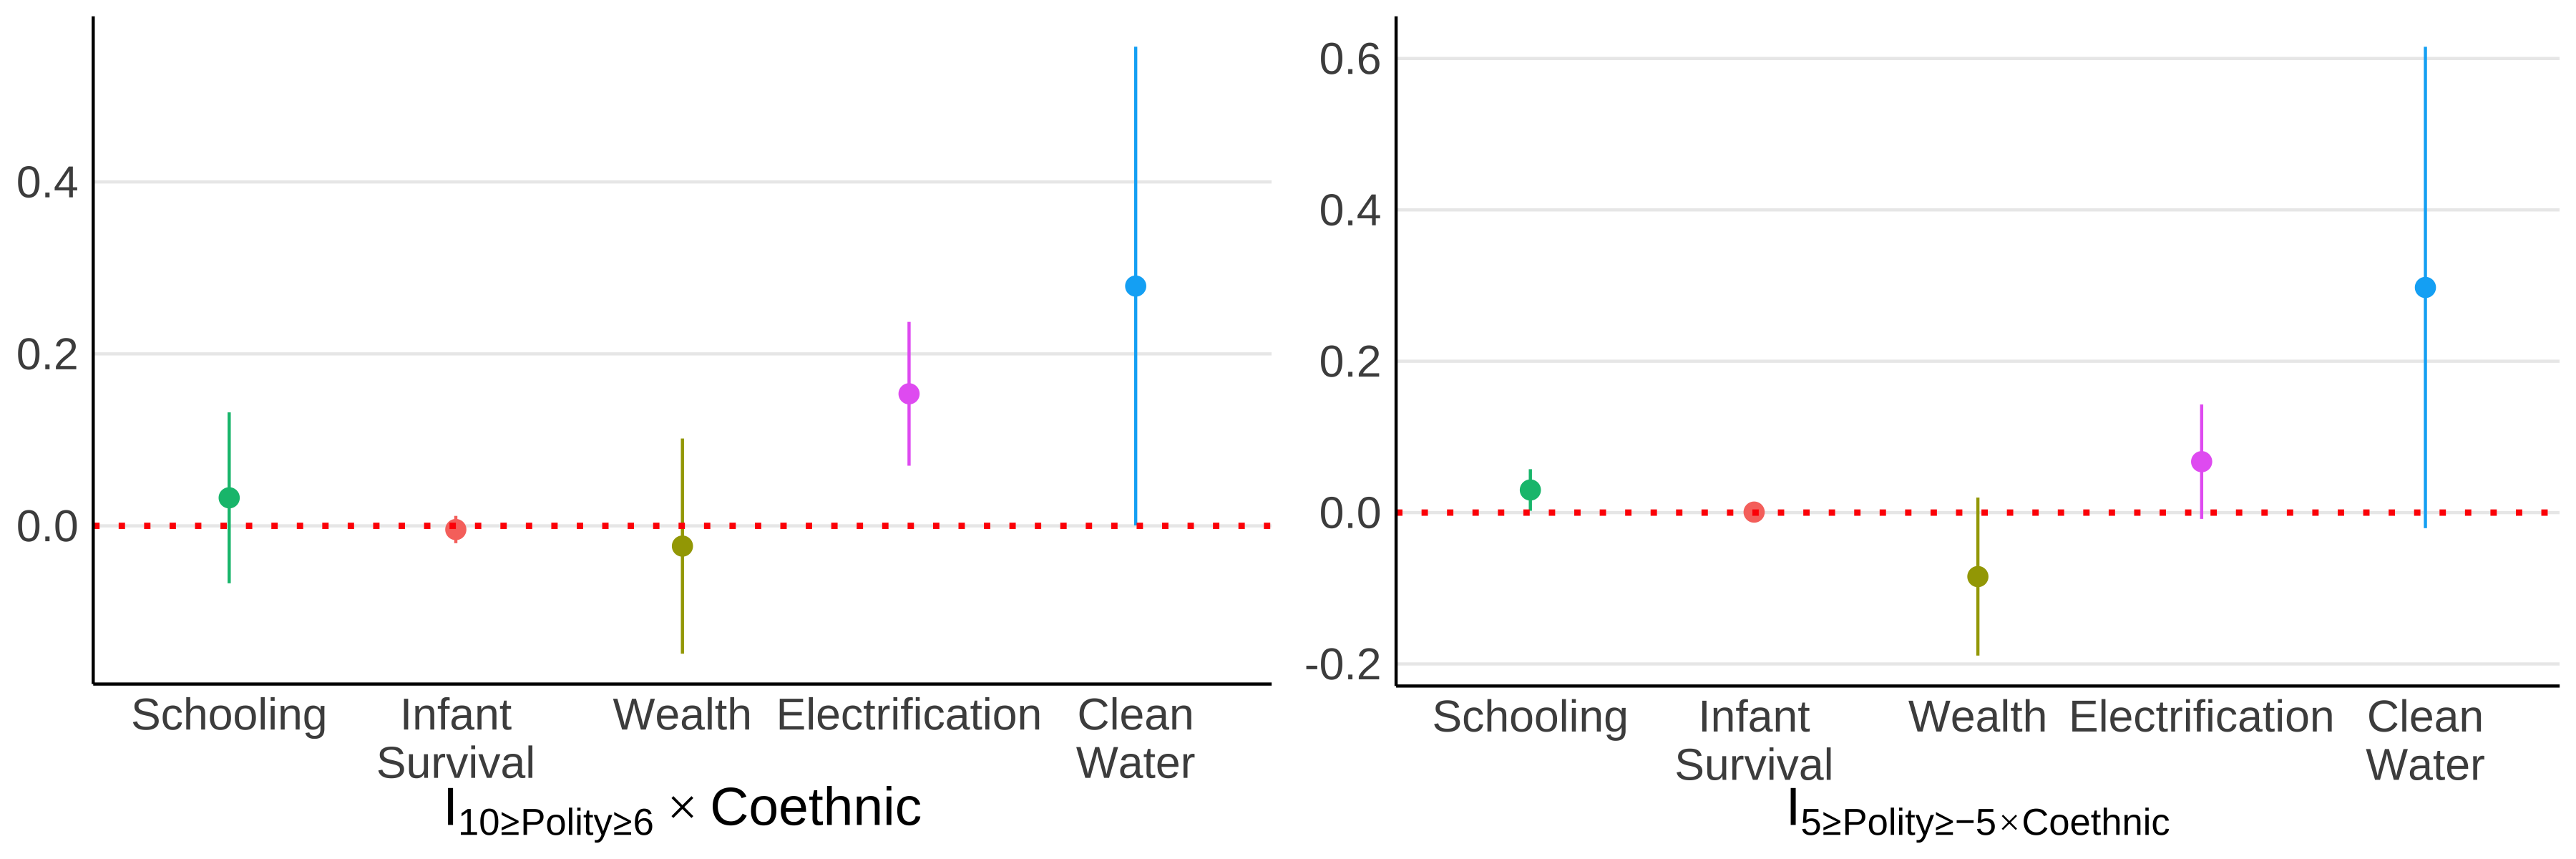
\includegraphics[width=.9\linewidth]{figure/coeth_dem_ethFE.png}
\caption{With ethnic groups and time fixed  effects.}
\label{fig:coedemet}
\note{In this figure, I present the effect of the interaction between co-ethnicity variable and Polity groups on primary school completion, infant survival, wealth, electrification and access to clean drinking water. Democracies have a \textit{Polity IV } $\in [10, 5]$, anocracies have a \textit{Polity IV } $\in [4, -5]$ and autocracies, the omitted group, have a \textit{Polity IV } $<-5$. The bands represent the 90\% confidence interval and the standard errors are clustered on ethnic groups. All estimates include ethnic group, time and age fixed effects.}
\end{figure}

Putting the result in context--- 36\% of non-co-ethnic observations in the sample had electricity. An ethnic kin in the most democratic countries would have an electrification rate of 51.4\%. Having more exposure to democracy increases ethnic favoritism in electrification. These results could be driven by the fact that leaders will now target funds to their ethnic group to earn their support in elections. Especially since the support of ethnic kins could come at a lower bill. Moreover, 77.6\% of non-co-ethnics finished primary school education while 80.6\% of co-ethnics in anocracies finished primary school education.

\subsection{Discussion}

The results from the previous sections capture, \textit{ceteris paribus}, the differences in outcomes between co-ethnic and non-co-ethnics. To interpret the results from the two previous sections as causal, I have to assume that the transitions between leaders of different ethnicities and in how democratic a country is are exogenous to the changes in an ethnic groups' education, health, electricity usage, wealth, and access to clean drinking water. A concern might arise from the fact that democracy is endogenous and is probably correlated with the outcomes I am studying. Even though the concern is correct, I am not interpreting the coefficient of democracy as a causal one. The coefficient of interest in this paper is that of the interaction between democracy and the co-ethnic variable. The coefficient of the interaction is less likely to suffer from an omitted variable bias. For the interaction between democracy and co-ethnicity to be endogenous, and thus have biased results, there must exist an omitted variable that is correlated with whether a country is a democracy, or not, and with how co-ethnics and non-co-ethnics are treated by their leaders. Such omitted variable is less likely to be found.

\begin{figure}[!htb]
\centering
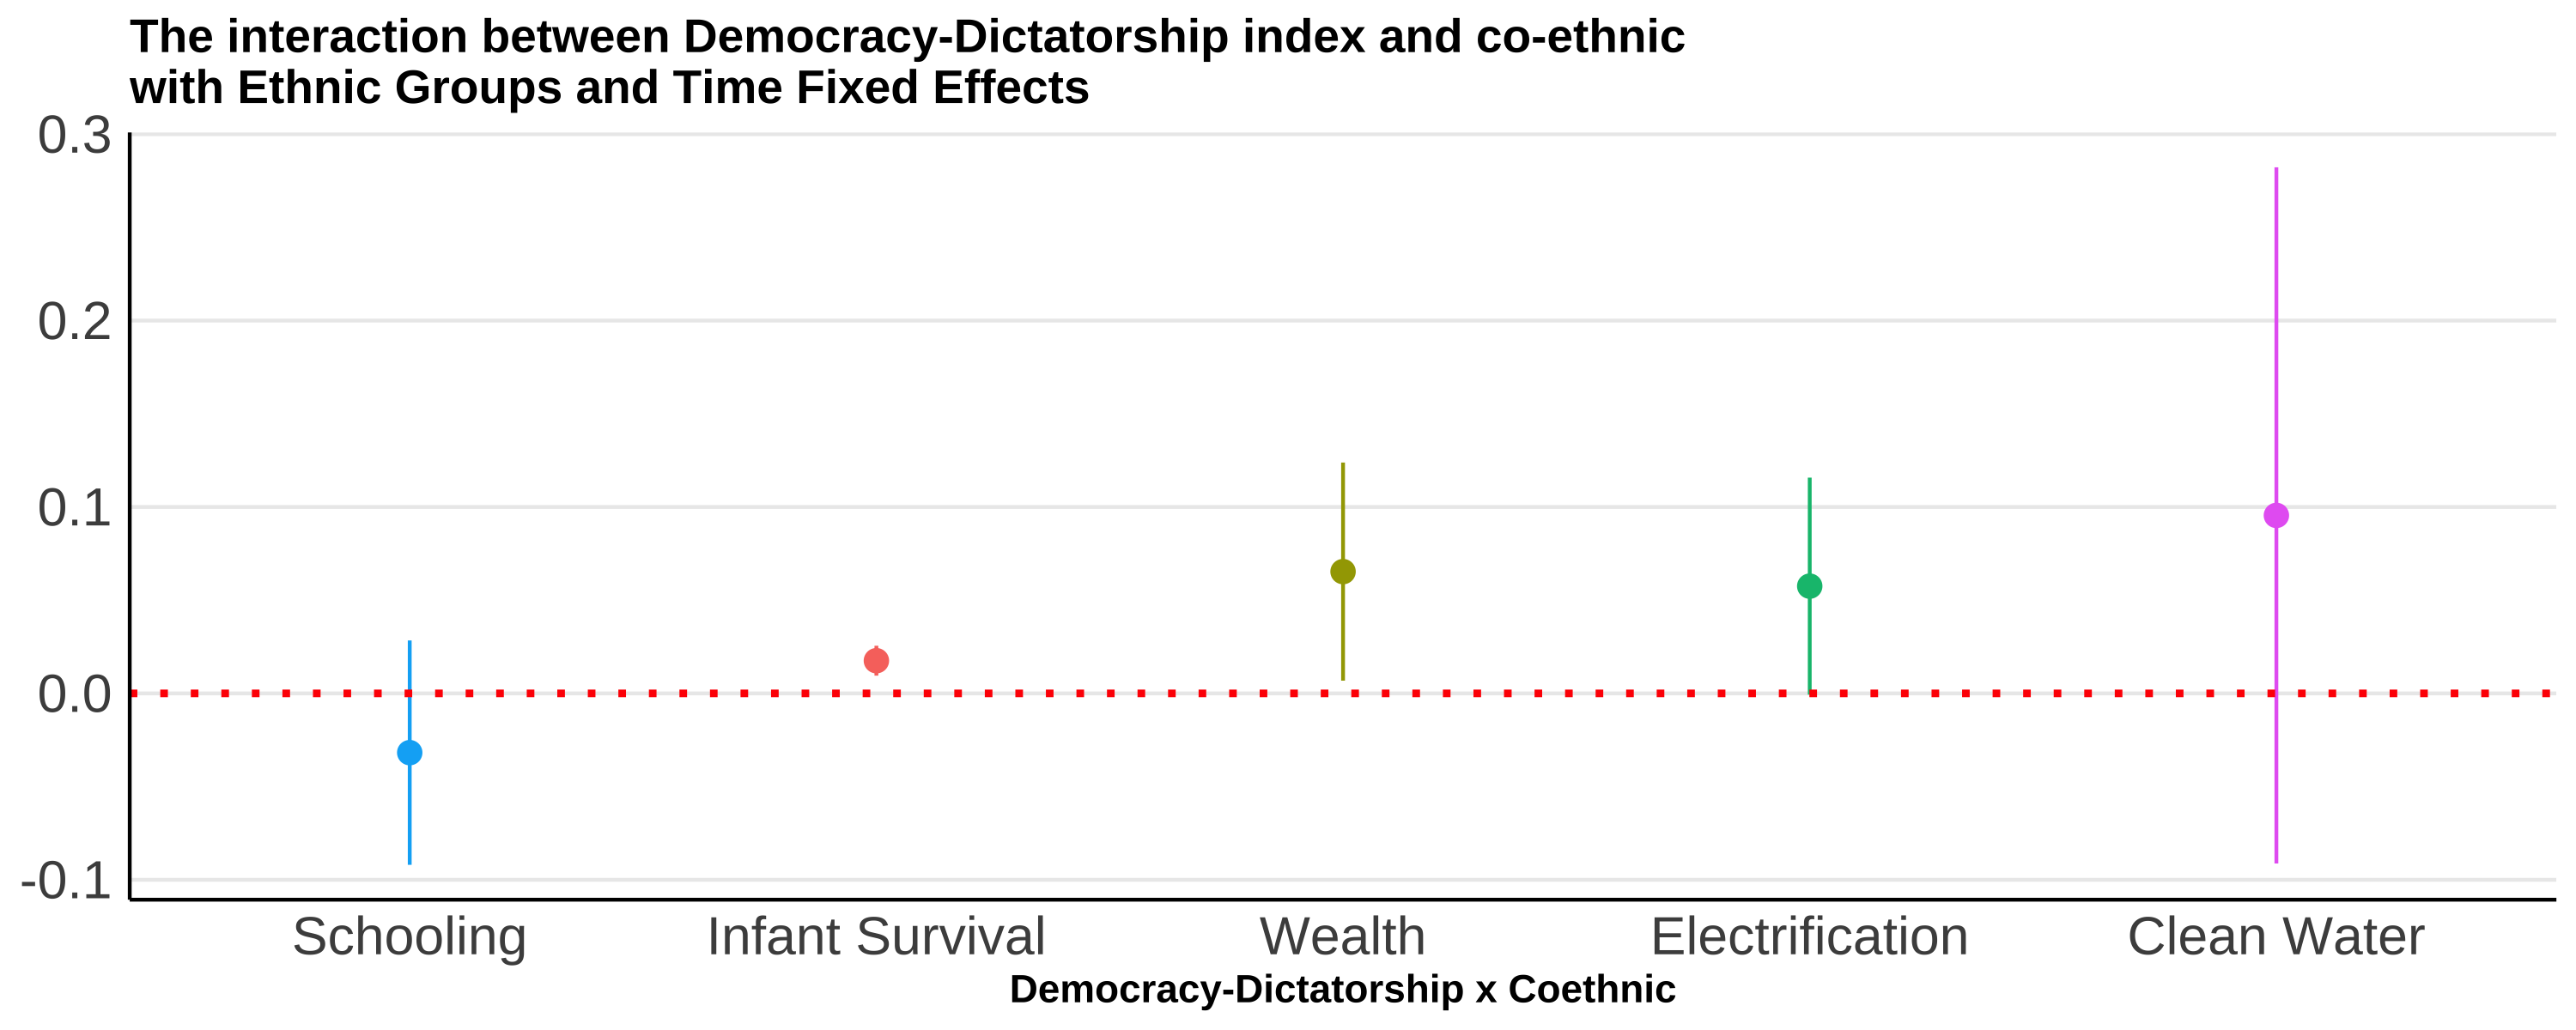
\includegraphics[width=.9\linewidth]{figure/coeth_demdic_ctFE.png}
\caption{Effect of the interaction between co-ethnicity and Democracy-Dictatorship Index on outcomes of interest with ethnic groups and time fixed effects.}
\label{fig:demdicindex}
\note{In this figure, I present the effect of the interaction between co-ethnicity variable and the Democracy-Dictatorship on primary school completion, infant survival, wealth, electrification and access to clean drinking water. In this specification, I used the Democracy-Dictatorship index as a measure of democracy. The Democracy-Dictatorship index is an indicator variable that is equal to 1 if a country is democratic and zero otherwise. The bands represent the 90\% confidence interval and the standard errors are clustered on ethnic groups. All estimates include ethnic group, time and age fixed effects.}
\end{figure}


Another concern could arise from the measure of democracy, \textit{Polity IV}, that I am using. Defining and quantifying the democratic institutions in a country is not straightforward and democracy differs from one country to another. My empirical strategy includes country and time-fixed effects. The inclusion of these fixed effects could alleviate the concern of the differences between democracy because it allows me to have a between and with-in country analysis. Moreover, the \textit{Polity IV} measure is developed based on five categories that aim to disentangle the differences in how more, or less, democratic a country is. Furthermore, I ran equation \ref{eq1} with a different measure of democracy. I used the \textit{Democracy-Dictatorship Index} instead of \textit{Polity IV}. The results to this regression are presented in table \ref{tab:ethdemdic} and figure \ref{fig:demdicindex}. Using the \textit{Democracy-Dictatorship Index}, I retrieved point estimates that have the same sign as these from the \textit{Polity IV} regression. The point estimates from the \textit{Polity IV} regression were significant for schooling in anocracies and electrification and access to clean drinking water in democracies and access wealth in anocracies. None of the results using the \textit{Democracy-Dictatorship Index} were significant. It could be the case that the coefficient of the effect of interaction between \textit{Democracy-Dictatorship Index} and co-ethnicity became insignificant because the \textit{Democracy-Dictatorship Index} lumps anocracies and democracies together, therefore the estimate will be averaging over both groups. 

\begin{table}[!h]

\caption{Ethnic favoritism and continuous democracy measure results. \label{tab:ethdemcont}}
\centering
\resizebox{\linewidth}{!}{
\begin{threeparttable}
\begin{tabular}[t]{lccccc}
\toprule
  & \specialcell{(1) \\ Schooling} & \specialcell{(2) \\ Infant Survival} & \specialcell{(3) \\ Wealth} & \specialcell{(4) \\ Electrification} & \specialcell{(5) \\ Clean Water}\\
\midrule
$PolityIV\times Coethnic$ & \num{0.01}* & \num{0.00} & \num{0.00} & \num{0.01}*** & \num{0.02}*\\
 & (\num{0.00}) & (\num{0.00}) & (\num{0.01}) & (\num{0.00}) & (\num{0.01})\\
\midrule
N & \num{1135494} & \num{2511731} & \num{750704} & \num{816320} & \num{816320}\\
Mean & \num{0.65} & \num{0.91} & \num{0.27} & \num{0.35} & \num{0.22}\\
Birth Year FE & X & X & X & X & X\\
Age FE & X & X & X & X & X\\
Country Specific Ethnic Group FE & X & X & X & X & X\\
\bottomrule
\multicolumn{6}{l}{\rule{0pt}{1em}* p $<$ 0.1, ** p $<$ 0.05, *** p $<$ 0.01}\\
\end{tabular}
\begin{tablenotes}
\item[1] \footnotesize{In this table, I am reporting the estimates of equation \ref{eq1}. 
                      I present the results of the interaction between the coethnic variable and 
                      \textit{Polity IV } groups on primary school completions in column 1, infant 
                      survival in column 2, wealth quintile in column 3, electrification in column 4 
                      and access to clean drinking water in column 4. Primary school completion is a 
                      dummy variable that is equal to one if a person completed primary school and 
                      zero otherwise. Infant survival is a dummy variable that is equal to one if an 
                      infant survived the first 12 months of life. Electrification is a dummy variable
                      that is equal to one if a household has electricity. Finally, access to clean 
                      drinking water is an ordinal variable that has values from 1, worst water source, to 4.}
\item[2] \footnotesize{\textit{Polity IV } score in this specification is continuous. It takes
                      values that range from most autocratic $-10$ to most democratic $10$}
\item[3] \footnotesize{Standard errors are clustered on ethnic groups. All 
                      results include ethnic group, time and age fixed effects.}
\end{tablenotes}
\end{threeparttable}}
\end{table}


\begin{table}[!h]

\caption{Ethnic favoritism and continuous democracy measure results. \label{tab:ethdemdic}}
\centering
\resizebox{\linewidth}{!}{
\begin{threeparttable}
\begin{tabular}[t]{lccccc}
\toprule
  & \specialcell{(1) \\ Schooling} & \specialcell{(2) \\ Infant Survival} & \specialcell{(3) \\ Wealth} & \specialcell{(4) \\ Electrification} & \specialcell{(5) \\ Clean Water}\\
\midrule
$D-DIndex\times Coethnic$ & \num{0.073} & \num{-0.008} & \num{0.111} & \num{0.057} & \num{-0.142}\\
 & (\num{0.058}) & (\num{0.007}) & (\num{0.074}) & (\num{0.037}) & (\num{0.112})\\
\midrule
Mean & \num{0.649} & \num{0.905} & \num{0.275} & \num{0.351} & \num{0.216}\\
N & \num{988262} & \num{2070052} & \num{452222} & \num{453673} & \num{453673}\\
\bottomrule
\multicolumn{6}{l}{\rule{0pt}{1em}* p $<$ 0.1, ** p $<$ 0.05, *** p $<$ 0.01}\\
\end{tabular}
\begin{tablenotes}
\item[1] \footnotesize{In this table, I am reporting the estimates of equation \ref{eq1}. 
                      I present the results of the interaction between the coethnic variable and 
                      \textit{Polity IV } groups on primary school completions in column 1, infant 
                      survival in column 2, wealth quintile in column 3, electrification in column 4 
                      and access to clean drinking water in column 4. Primary school completion is a 
                      dummy variable that is equal to one if a person completed primary school and 
                      zero otherwise. Infant survival is a dummy variable that is equal to one if an 
                      infant survived the first 12 months of life. Electrification is a dummy variable
                      that is equal to one if a household has electricity. Finally, access to clean 
                      drinking water is an ordinal variable that has values from 1, worst water source, to 4.}
\item[2] \footnotesize{\textit{Polity IV } score in this specification is continuous. It takes
                      values that range from most autocratic $-10$ to most democratic $10$}
\item[3] \footnotesize{Standard errors are clustered on ethnic groups. All 
                      results include ethnic group, time and age fixed effects.}
\end{tablenotes}
\end{threeparttable}}
\end{table}


Another concern could be the ``psychic effect'' of having a co-ethnic person as the leader of a country. The ``psychic effect'' implies that a person will have better outcomes because ethnic kin became a leader without intervention by the leader herself. For example, \citet{marx2009obama} find that test scores of African American children in the US improved following the election of Barack Obama. The authors argue that the increase in test scores does not reflect an allocation of resources that targeted African American pupils but the greater motivation of having a role model in an important position. The ``psychic effect'' is unlikely to cause a sudden increase in electrification and access to clean drinking water without the allocation of resources to benefit one ethnic group. Just because a leader is of a specific ethnic group will not magically create an infrastructure that delivers electricity and clean drinking water. The ``psychic effect'', however, can influence education, health and wealth. To address this concern I use the nightlight used by \citet{hodler2014regional} to show the existence of regional favoritism. I restrict the dataset to the countries I use in my DHS sample. I run the following regression:

\begin{equation}\label{eq:hodler}
Light_{ict} = \alpha_{ic} + \lambda_{ct} + \beta_{1}Leader_{ict}\times Polity_{ct} + \beta_{2}Leader_{ict} + \beta_{3} Polity_{ct} + \epsilon_{ict}
\end{equation}

Where $Light_{ict}$ is the log of the average nighttime light intensity in ethnographic region $i$ in country $c$ at time $t$ \footnote{following \citet{henderson2012measuring,michalopoulos2014national,michalopoulos2013pre,hodler2014regional,hodler2014economic}, the nighttime intensity variable is in logs after adding 0.01 because the distribution of light is right-skewed.}. The variable $\alpha_{ic}$ is a region-fixed effect that controls for regional characteristics that vary across time, like historical and climatic factors. $\lambda_{ct}$ is a vector of country-year dummy variables that would serve as a control for regional shocks and changes to satellites and sensory deterioration. \citet{henderson2012measuring} document a strong correlation between a country's GDP and nighttime light intensity. Therefore, $Light_{ict}$ could reflect the economic condition in a country, which is associated with education, health and wealth---the outcomes of interest I am studying. 

\begin{center}
\begin{table}[H]
\centering
\caption{Institutions' effects on ethnic \\ favoritism: using light data.}
\label{tab:hodler}
\begin{tabular}{lcccccccc}
\hline 
 & \multicolumn{3}{c}{Ethnologue} &  &  & \multicolumn{3}{c}{GREG}\tabularnewline
\cline{2-4} \cline{7-9} 
 &  & $Light_{ict}$ &  &  &  &  & $Light_{ict}$ & \tabularnewline
\hline 
\textbf{Panel A: Ethnic Favoritism} &  &  &  &  &  &  &  & \tabularnewline
$Coethnic_{ict}$ &  & 0.061 &  &  &  &  & 0.097{**} & \tabularnewline
 &  & (0.051) &  &  &  &  & (0.036) & \tabularnewline
\textbf{Panel B: Ethnic favoritism} &  &  &  &  &  &  &  & \tabularnewline
\textbf{and institutions} &  &  &  &  &  &  &  & \tabularnewline
$Coethnic_{ict}\times Polity_{ct}$ &  & -0.076 &  &  &  &  & -0.041 & \tabularnewline
 &  & (0.204) &  &  &  &  & (0.131) & \tabularnewline
%$Coethnic_{ict}\times Anocracy_{ct}$ &  & 0.192{*} &  &  &  &  & 0.027 & \tabularnewline
% &  & (0.090) &  &  &  &  & (0.773) & \tabularnewline
\hline 
\end{tabular}
\end{table}
\end{center}

Using the data from \citet{hodler2014regional} allows me to detect regional favoritism when a leader would allocate resources to regions where her ethnic group lives. The ``psychic effect'' or the ``Obama effect'' will not influence the results of regional favoritism because when a leader is targeting one region, they cannot exclude specific ethnic groups that live in said region. The results to equation \ref{eq:hodler} are presented in table \ref{tab:hodler}. In panel A, I present the results of the existence of regional favoritism, while in panel B I present the results when I interact the leader's ethnicity with \textit{Polity IV}. The results are similar to what I found in my analysis of the interaction between \textit{Polity IV} and co-ethnicity.

% \begin{table}[H]
%   \centering
%   \renewcommand*\TPTnoteLabel[1]{\parbox[b]{3em}{\hfill#1\,}}
%   \begin{threeparttable}
% \caption{\textsc{Ethnic favoritism results by Polity IV group.}}\label{tab:grps}
% \footnotesize
%  \begin{tabular}{l c c c c c}
%   \hline
%   %\toprule%\rowstyle{\bfseries}
%    &Schooling & Infant Survival & Electrification & Water  & Wealth\\
%   \midrule

%   \makecell[l]{\textit{\textbf{Panel A}}} \\
%   Democracy &  -0.029 	& 0.003 & 0.055*** & -0.053* & 0.107***\\
%   					& (0.022)	& (0.006) & (0.021) & (0.032) & (0.037)\\
%     \makecell[l]{\textit{\textbf{Panel B}}} \\
%   Anocracy 	& -0.30* 	& 0.010 & 0.008 & 0.015 & -0.033\\
%   					& (0.015)	& (0.006) & (0.018) & (0.079) & (0.150)\\
%     \makecell[l]{\textit{\textbf{Panel C}}} \\
%   Autocracy 	& -0.045* 	& 0.007 & -0.036 & 0.391** & 0.086\\
%   					& (0.027)	& (0.008) & (0.023) & (0.189) & (0.081)\\
% \bottomrule
%   \end{tabular}
%   \begin{footnotesize}
%   \begin{tablenotes}[normal,flushleft]
%     \item[1] In this table, I am reporting the estimates of equation \ref{eqFR1} individually for democracies, anocracies and autocracies. I present the results of the effect of ethnic favoritism on primary school completions in column 1, infant survival in column 2, wealth quintile in column 3, electrification in column 4 and access to clean drinking water in column 4. Primary school completion is a dummy variable that is equal to one if a person completed primary school and zero otherwise. Infant survival is a dummy variable that is equal to one if an infant survived the first 12 months of life. Electrification is a dummy variable that is equal to one if a household has electricity. Finally, access to clean drinking water is an ordinal variable that has values from 1, worst water source, to 4.
%     \item[2] Standard errors are clustered on ethnic groups. All results include ethnic group, time and age fixed effects.
%            \end{tablenotes}
%            \end{footnotesize}  
%            \end{threeparttable}
% \end{table}

% I need to falsify the co-ethnic variable and let it date back a few years early


%Ethnic favoritism could negatively affect the economy. It could increase inequality along the ethnic lines \citep{easterly1997africa} and could lead to lower growth. Therefore, investigating the effect of checks and balances on ethnic favoritism is important. To analyze the effect of institutions on ethnic favoritism, I will use \ref{eq3}. The empirical specification allows for heterogeneity in democratic treatment, taking advantage of \textit{Polity IV}. I divided countries into groups. I constructed these groups using five points intervals. Then I constructed the failed or occupied group. This specification is given by equation \ref{eq2}, with the least democratic group--- the most autocratic countries--- as the omitted variable. I present the results in table \ref{tab:ethdem} and figure \ref{fig:coedemet}.
%
%\begin{equation}\label{eq3}
%\begin{split}
%    Y_{ietag} &= \beta_{0} + \beta_{1}coethnic_{ietag} + \sum_{k} \beta_{k}coethnic_{ietag} \cdot I_{(k-1\leq Polity IV \leq k)} \\
%    &+ \delta_{t} + \gamma_{e}+\eta_{a} + \lambda_{g} + \varepsilon_{ict}
%\end{split}
%\end{equation}
%
%In table \ref{tab:ethdem} column 1, I present the results of regressing primary school completion on the interaction between the different polity bins and coethnicity. The results show that the difference between coethnics and non-coethnics is the same in democracies and autocracies, closed-anocracies and autocracies. A coethnic in a democracy/closed-anocracy has the same chance of completing primary school when compared to a coethnic in a dictatorship. The results change when comparing coethnics and non-coethnics in open-anocracies and autocracies. The difference between coethnics and non-coethnics in open-anocracies and autocracies is 7.0\%.
%
%Moreover, I show the results when considering the effect of institutions on infant mortality in table \ref{tab:ethdem} column 2. The difference between coethnics and non-coethnics is 0.9\% in democracies versus autocracies. A positive difference indicates a disadvantage, where an infant is more likely to die during his/her first 12 months of living. Coethnics and non-coethnics in closed-anocracies versus autocracies and open-anocracies versus autocracies are statistically the same. 
%
%Wealth is another outcome that is interesting to study in the context of ethnic favoritism and institutions. When I considered wealth as the output of interest, the difference between coethnics and non-coethnics in democracies and dictatorships was 0.072. In other words, democracy increased ethnic favoritism where the wealth of individuals that lived under the rule of a co-ethnic leader during the four years before the interview and lived in a democratic country had higher wealth than those that lived under the rule of a despotic coethnic leader. However, the difference between coethnics and non-coethnics in closed-anocracies versus autocracies, and open-anocracies versus autocracies is -0.063 and -0.108 respectively. Therefore, ethnic favoritism decreases when comparing coethnics and non-coethnics in closed-anocracies/open-anocracies and autocracies. 
%
%
%The results of the interaction between democracy and the coethnicity variable on electrification are presented in column 4 of table \ref{tab:ethdem}. The difference between coethnics and non-coethnics is positive---ethnic-favoritism exists--- when comparing democracies, open-anocracies and close-anocracies to autocracies. The differences are 15.1\%, 9.3\% and 5.3\% respectively.
%
%Since water scarcity and access to clean drinking water is an important issue in Africa. I use the data collected by the DHS on access to water as another outcome of interest. The results showed that the difference between coethnics and non-coethnics in democracies/open-anocracies/close-anocracies are positives. Therefore, coethnics have better access to water.

\section{Conclusion}\label{sec6}
Ethnic favoritism and inequitable distribution of resources could be holding back the growth of some African countries \citep{easterly1997africa, alesina2005ethnic}. Institutions could also play a part in explaining why African countries lagged behind other nations \citep{acemoglu2001colonial, alsan2015effect}. This paper's results further show that ethnic diversity and corruption could be one of the causes of Africa's slow growth. 

When studying the effect of ethnic favoritism, I find that people that spent all of their primary school when a leader was co-ethnic were 3.8 percentage points less likely to finish primary school, though the result was statistically insignificant. A child whose mom shared the same ethnicity as the leader of the country she lived in two years before birth is 1.3 percentage points more likely to survive the first 12 months of birth. Co-ethnics were as likely as their non-co-ethnic peers to be in the same wealth quintile and have electricity, though the results are statistically insignificant. Finally, co-ethnics have better access to clean drinking water than non-co-ethnics.

When I allow for the heterogeneous effect of democracy, the interaction between democratic bins and co-ethnicity are statistically significant when studying their effect on electrification and access to clean drinking water in democracies and anocracies and schooling among anocracies. Co-ethnicity and more democracy do not eliminate ethnic favoritism when it comes to primary infant survival and access to clean drinking water. Co-ethnics in democracies are as likely to finish primary schooling and survive the first year of birth as their non-co-ethnic peers. Co-ethnics in anocracies are 3 percentage points more likely to finish primary school. However, Co-ethnics in democracies are 15.4 percentage points more likely and anocracies are 6.7 percentage points more likely to have electricity. People living under the rule of co-ethnic kin in democracies and anocracies are more likely to have cleaner drinking waters. The results I find are consistent with the empirical work of \citet{kramon2013benefits} and the theoretical work of \citet{francois2015power}. Where evidence of ethnic favoritism depends on the outcome one studies and that autocracies in Africa are more ethnically representative than western democracies. Leaders aim to stay in power, to do so they will have to share the benefits of being a leader.


\pagebreak
\bibliography{ethnicfav}
\pagebreak
\nocite{*}

\begin{appendices}


%\begin{table}[!htbp]
%\caption{Effect of ethnic favoritism on variables of interest by Polity IV group.} \label{tab:ethgrps}
% \estwide{ethnic_fav_grps.tex}{10}{lccccc}
%\end{table}

\section{Data Appendix}

\begin{table}[!htb]
\caption{The number of co-ethnic and non-coethnic observations in each polity score.}
\label{tab5}
\resizebox{\textwidth}{!}{%
\begin{tabular}{l|ll}
Polity Score & \begin{tabular}[c]{@{}l@{}}Not a \\ Co-ethnic Leader\end{tabular} & Co-ethnic Leader \\ \hline
-9           & 130,381                                                          & 26,648          \\
-8           & 27,207                                                           & 1,613           \\
-7           & 241,663                                                          & 37,388          \\
-6           & 37,936                                                           & 3,701           \\
-5           & 17,965                                                           & 5,928           \\
-4           & 23,396                                                           & 1,564           \\
-3           & 12,863                                                           & 3,147           \\
-2           & 9,870                                                            & 1,338           \\
-1           & 44,950                                                           & 19,604          \\
0            & 16,269                                                           & 1,336           \\
1            & 6,624                                                            & 340             \\
2            & 6,345                                                            & 200             \\
3            & 7,604                                                            & 273             \\
4            & 31,825                                                           & 1,689           \\
5            & 4,550                                                            & 539             \\
6            & 13,091                                                           & 3,329           \\
7            & 18,290                                                           & 4,054           \\
8            & 5,890                                                            & 1,674           \\
9            & 37                                                               & 1,762          
\end{tabular}%
}
\end{table}

\newpage
\begin{table}[!htb]
\caption{The number of co-ethnic and non-coethnic observations in polity groups.}
\label{tab6}
\resizebox{\textwidth}{!}{%
\begin{tabular}{l|ll}
Polity Score       & \begin{tabular}[c]{@{}l@{}}Not a \\ Co-ethnic Leader\end{tabular} & Co-ethnic Leader \\ \hline
Democracy          & 37,308                                                           & 10,819          \\
Open Anocracy      & 56,948                                                           & 3,041           \\
Closed Anocracy    & 125,313                                                          & 32,917          \\
Autocracy          & 437,187                                                          & 69,350          \\
Failed or Occupied & 1,229                                                            & 92             
\end{tabular}%
}
\end{table}

\subsection{Countries included in the data-set}
I used data from twenty-one countries. These countries and the distribution of observations are presented in table \ref{countries}.

\begin{table}[!htb]
\centering
\caption{Number of Observations by country.}
\label{countries}
\resizebox{\textwidth}{!}{%
\begin{tabular}{@{}lll@{}}
\toprule
Country                   & Number of observations & Percent \\ \midrule
Angola                    & 12,145                 & 1.57    \\
Cameroon                  & 31,777                 & 4.10    \\
Congo Democratic Republic & 28,224                 & 3.65    \\
Benin                     & 41,969                 & 5.42    \\
Ethiopia                  & 29,437                 & 3.80    \\
Ghana                     & 27,571                 & 3.56    \\
Guinea                    & 22,107                 & 2.86    \\
Cote d'Ivoire             & 18,403                 & 2.38    \\
Kenya                     & 58,278                 & 7.53    \\
Malawi                    & 68,081                 & 8.79    \\
Mali                      & 42,372                 & 5.47    \\
Mozambique                & 18,179                 & 2.35    \\
Namibia                   & 2,872                  & 0.37    \\
Niger                     & 29,963                 & 3.87    \\
Nigeria                   & 90,445                 & 11.68   \\
Senegal                   & 92,990                 & 12.01   \\
South Africa              & 20,249                 & 2.62    \\
Zimbabwe                  & 16,987                 & 2.19    \\
Uganda                    & 47,739                 & 6.17    \\
Burkina Faso              & 36,834                 & 4.76    \\
Zambia                    & 37,582                 & 4.85    \\ \hline
Total                     & 774,204                & 100     \\ \bottomrule
\end{tabular}%
}
\end{table} 
\end{appendices}
\end{document}
